\section{Introduction}

In the following report we present the development of a software 
solution for the visuzalisation and the kinematic analysis of the 
exoskeleton hand shown in Fig. \ref{fig:exoskeleton_assembly}. The proposed 
design has been the result of the combined work of Tj A. Taiwo and Antonia
Tzemanaki. A detailed description of the exoskeleton and its design can be found 
in the handover report of TJ A. Taiwo \cite{tj_a_taiwo_exoskeleton_2021} and
in the doctoral thesis of Antonia Tzemanaki
\cite{tzemanaki_anthropomorphic_nodate}, included with this document.
In the following chapters we analyze the integration of the existing hardware 
with different software solutions for the visuzalisation of the exoskeletons 
kinematic behaviour. We also present the development of features and tools 
that fascilitated the manufacturing process of the exoskeleton.
\begin{figure}[h]
    \centering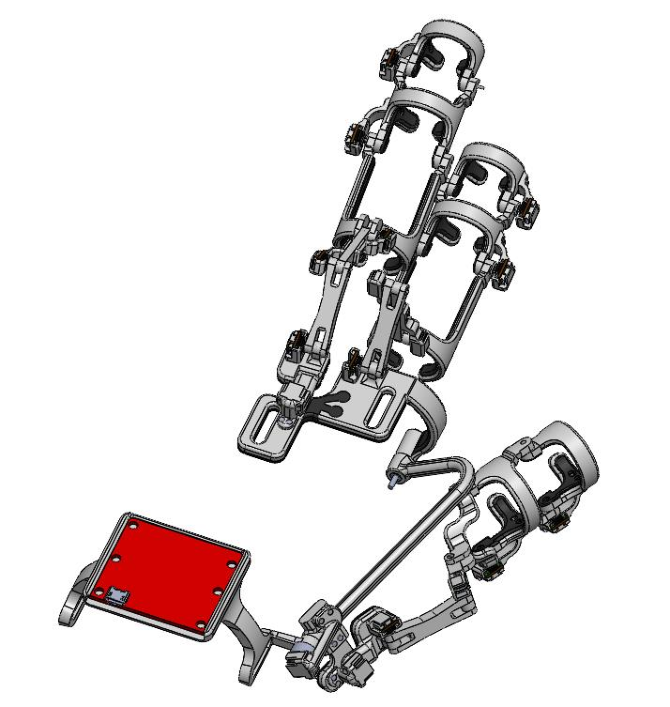
\includegraphics[width=0.65 \linewidth]{Figures/white_exoskeleton.pdf}
    \caption{Exoskeleton assembly.}
    \label{fig:exoskeleton_assembly}
\end{figure}

\section{Hand Measurements}
In \cite{tj_a_taiwo_exoskeleton_2021} a detailed description of the exoskeleton's 
design and assembly is presented. One of the key features of the design is 
that it allows the parametric definition of its dimensions based on the user's
hand measurements. This is made possible with the help of a set of equations that 
define the hand's geometry as a function of some characteristic lengths.
As described in \cite{tj_a_taiwo_exoskeleton_2021}, these 
lengths are defined in the
\texttt{\href{https://tinyurl.com/5ej3n2ud}{"equation.txt"}} file and they are
automatically parsed by the software (Solidworks). To fascilitate the process
of generating 
the \texttt{\href{https://tinyurl.com/5ej3n2ud}{"equation.txt"}} file a
simple Python script was created. The script reads 
the user's hand measurements using the
\texttt{\href{https://tinyurl.com/54d6zw5b}{"Exoskeleton Hand Measurements\_AT.xlsx"}}
file and automatically produces the
\texttt{\href{https://tinyurl.com/5ej3n2ud}{"equation.txt"}} file. The template
used for storing the user's hand measurements is shown in
Fig. \ref{fig:hand_measurements_template}.
A detailed description of the measurements names shown in Fig.
\ref{fig:hand_measurements_template} and how to take them is given
in \cite{tj_a_taiwo_exoskeleton_2021}. 
\begin{figure}
    \centering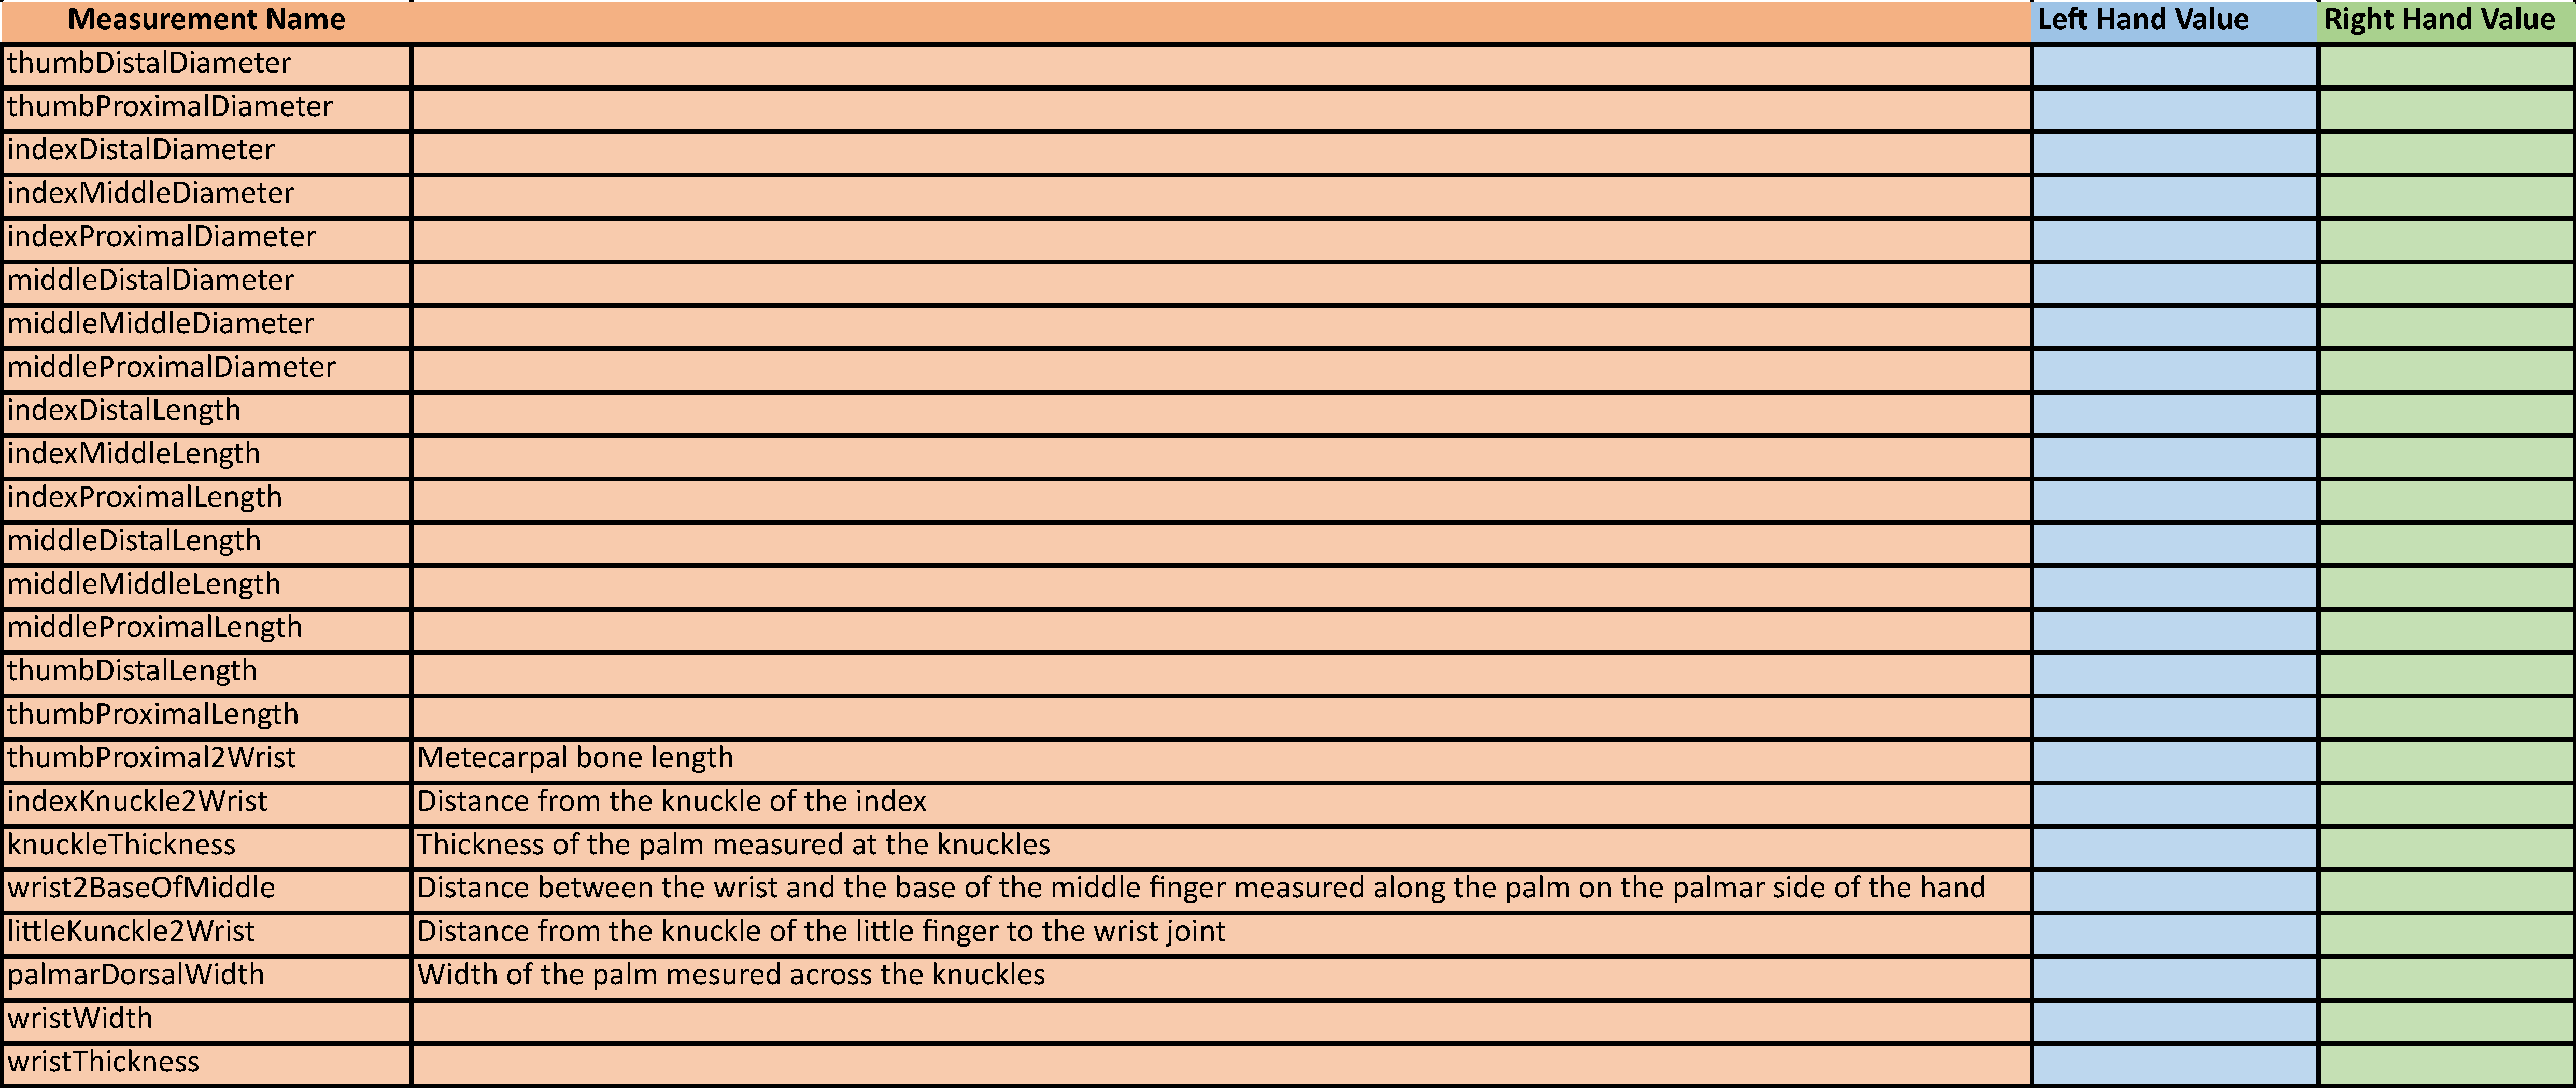
\includegraphics[width=1.0 \linewidth]{Figures/handmeasurements_template.pdf}
    \caption{Template format for storing the user's hand measurements.}
    \label{fig:hand_measurements_template}
\end{figure}

To generate the equation file the user needs to create a new tab in the 
provided Excel file 'Exoskeleton Hand Measurements AT'. Then
by executing the provided application
\texttt{\href{https://tinyurl.com/mrjjk566}{"hand\_parameters.exe"} } or the 
the associated Python script
\texttt{\href{https://tinyurl.com/yjefhtxr}{"hand\_parameters.py"}},
the user can automatically generate the required 
equations file. The application has a command line interface, as shown in 
Fig. \ref{fig:hand_measurements_application}, where the user inserts
the name of the tab as well as whether measurements are intented for the
left or the right hand.
\begin{figure}[h]
    \centering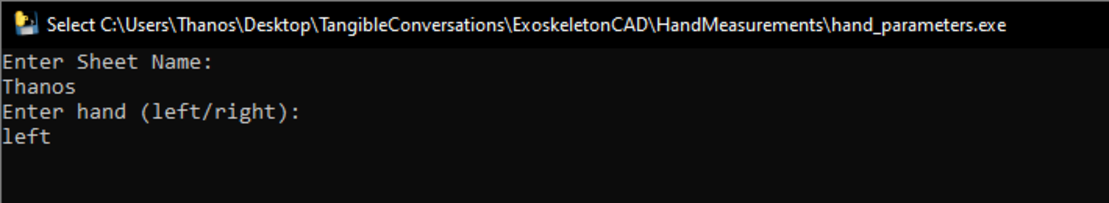
\includegraphics[width=1.0 \linewidth]{Figures/hand_measurements_script.pdf}
    \caption{Hand measurements application.}
    \label{fig:hand_measurements_application}
\end{figure}
To execute the files please first make a local copy of the 
\texttt{\href{https://tinyurl.com/2p9ar4a3}{HandMeasurements}} folder.

\section{Electronics and Hardware}
As discussed in \cite{tj_a_taiwo_exoskeleton_2021} the exoskeleton uses 
magnetic rotary encodes to measure the hand's joint angles.
In this project we use the
\texttt{\href{https://tinyurl.com/2rdkw8fr}{Melexis 90316}}
absolute rotary encoder. The sensors need to be calibrated with the 
help of specialist equipment in the BRL.

\subsection{Melexis Custom PCB}
The Melexis sensors are soldered onto a
\texttt{\href{https://tinyurl.com/46496kpn}{custom PCB}} made by Jason Welsby
(BRL Technician). The files can be viewed and processed with the 
help of Autodesk Eagle. The custom PCB enables the daisy chaining of the 
Melexis sensors. Each PCB has the option to connect one of two
“zero ohm resistors” which routes the signal coming from the sensor either to
the OUT1 or OUT2 channel of the JST connector attached to the PCBs
underside, see Fig. \ref{fig:melexis_board}. The JST connectors are wired so a
cable can be plugged into either side of the board. For daisy chaining to
work a PCB with the OUT1 signal needs to be connected to a PCB with the
OUT2 signal, otherwise the sensors output will interfere will each other
providing inaccurate data. To seperate the PCB's we color code them to 
green and red. Thus, a green sensor can only daisy chained to a red sensor. 
Sensors of the same color can not be connected together. To color code a 
sensor a microscope might be necessary. Please, ask Jason Welsby for more
information.
\begin{figure}[t]
    \centering
        \subfloat[Melexis custom PCB wiring.]{
        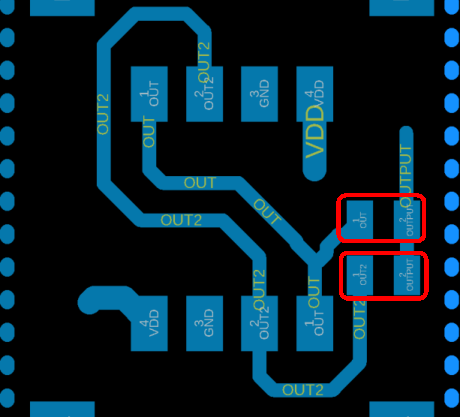
\includegraphics[width=0.45\textwidth]{Figures/melexis_board.pdf}
        \label{fig:melexis_board}
    }
    \qquad
    \subfloat[Custom PCB board and ports numbering convention.]{
        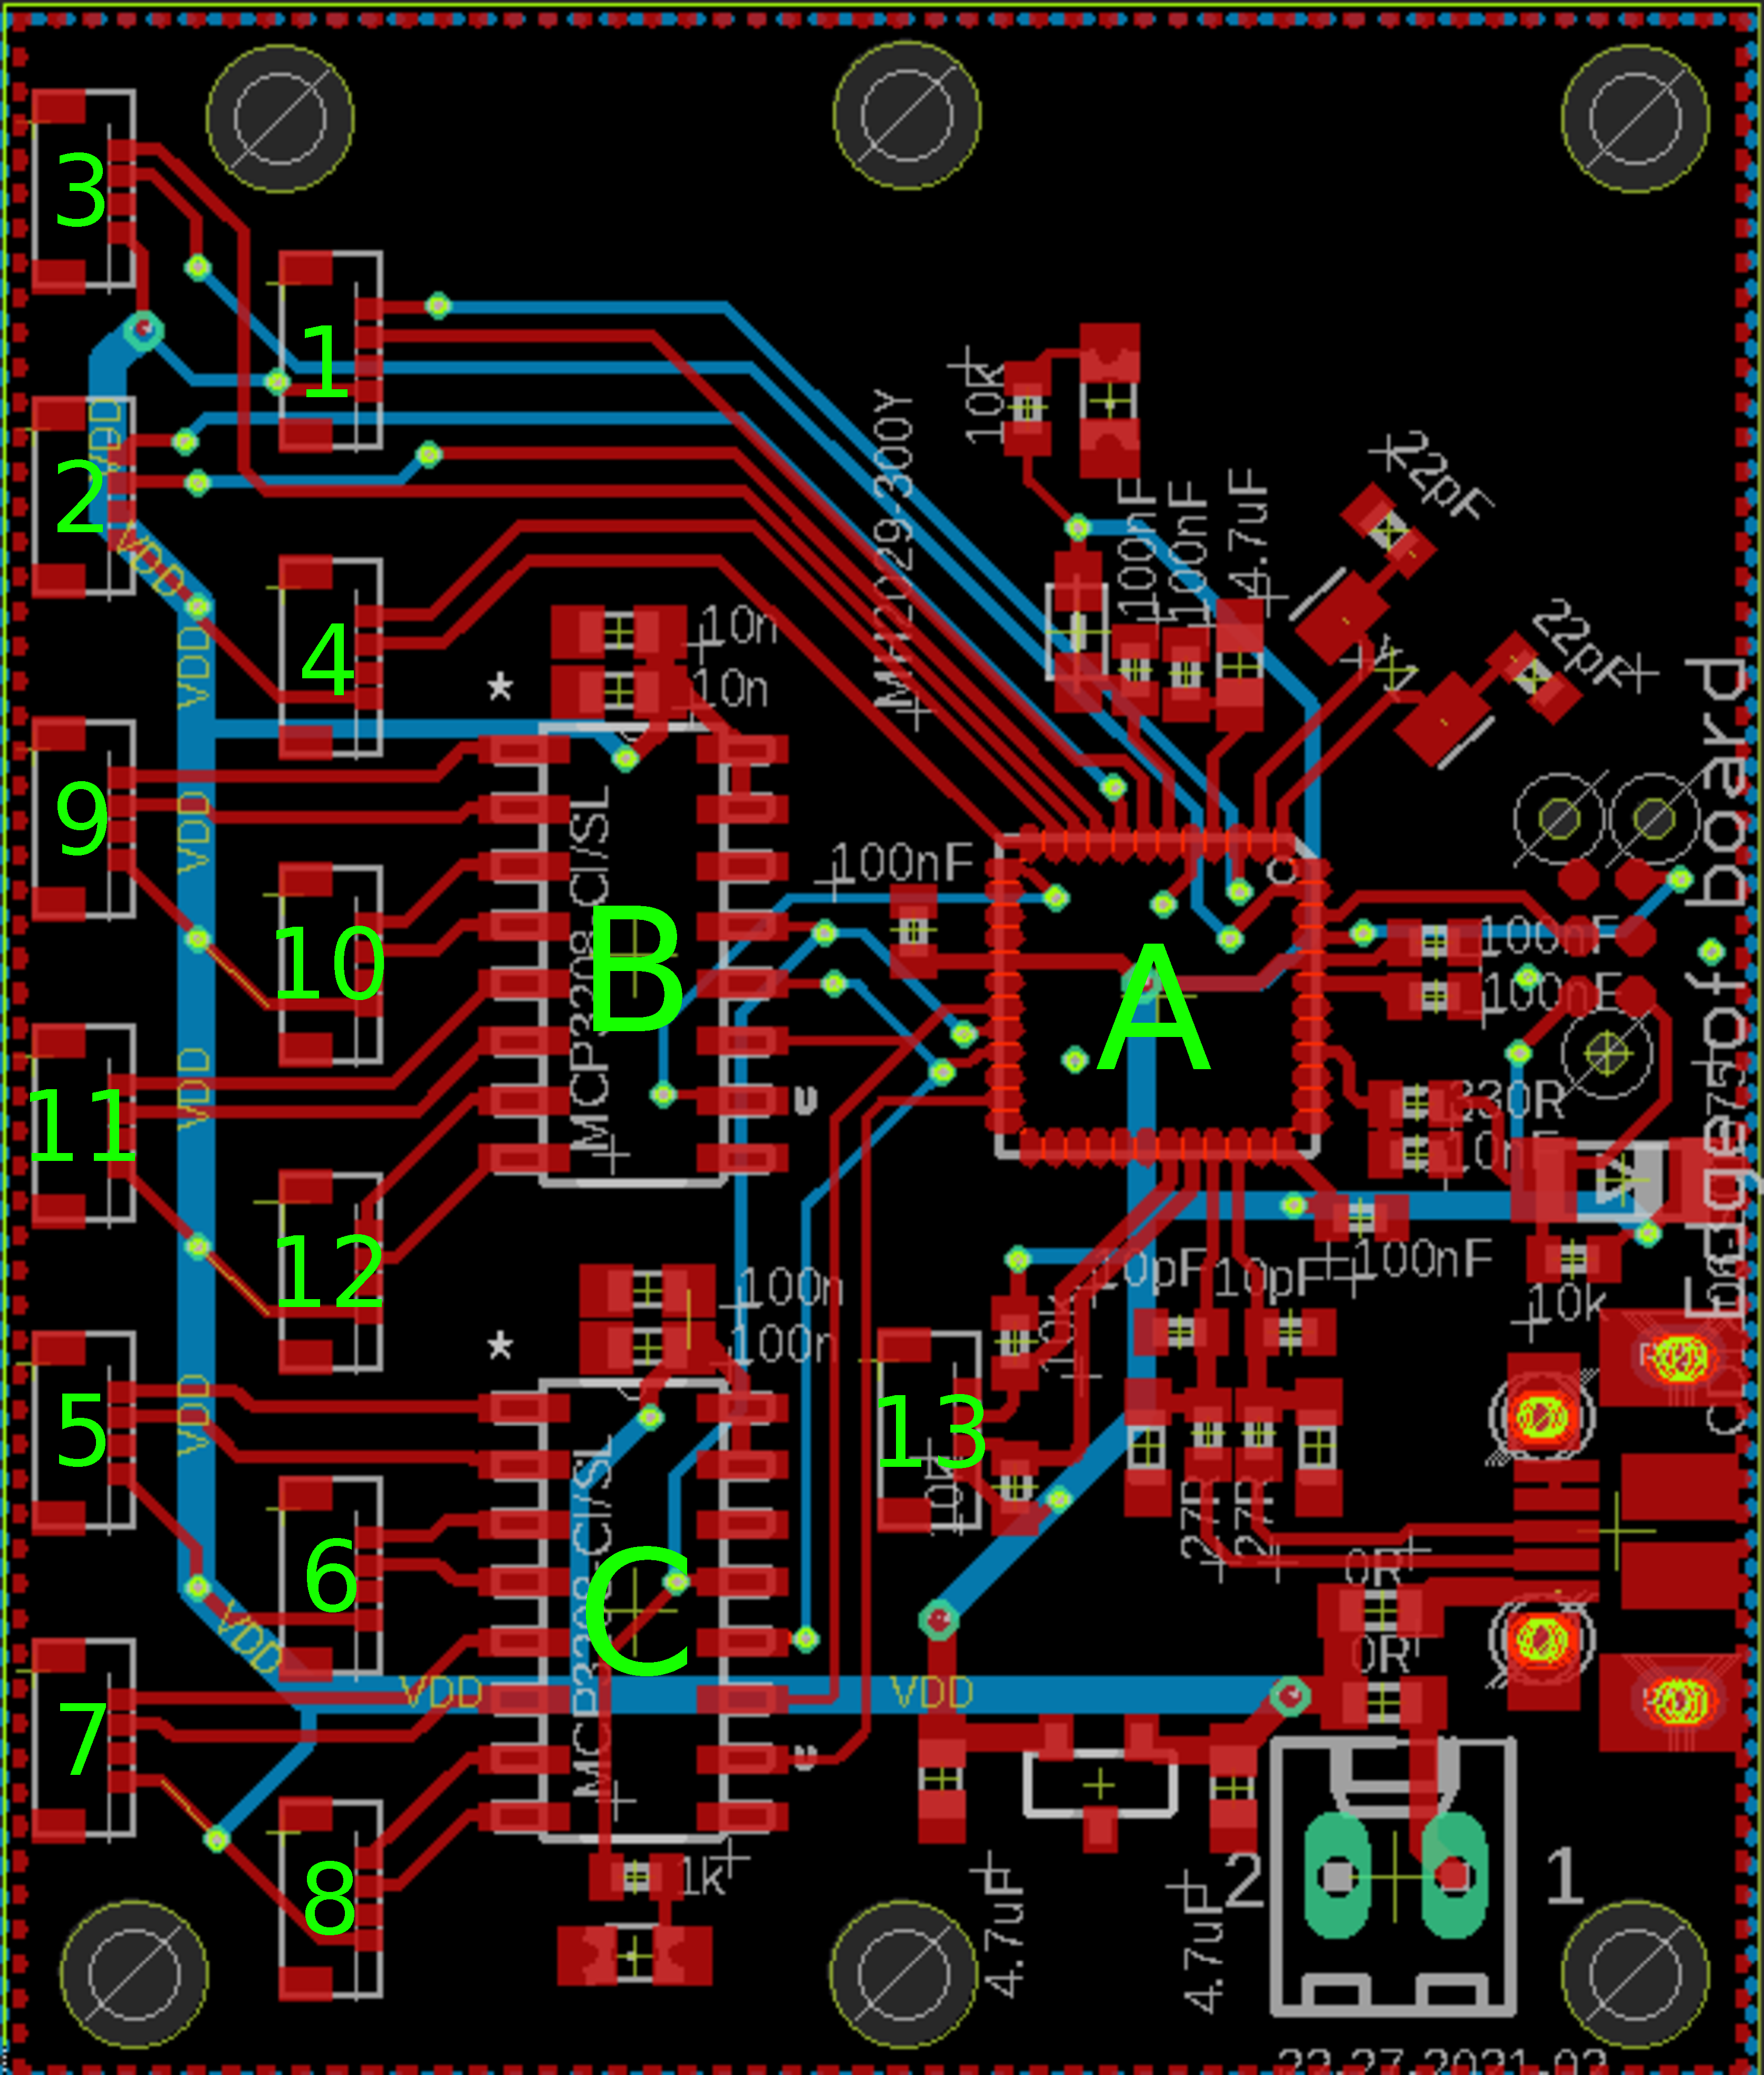
\includegraphics[width=0.45\textwidth]{Figures/custom_board.pdf}
        \label{fig:pcb_board}
    }
    \caption{Custom PCBs for the Melexis sensor and the exoskeleton's circuit board.}
    \label{fig:pcbs}
\end{figure}

\subsection{Mainboard}
The mainboard for the exoskeleton project was custom made by Jason Welsby 
and its design is shown in Fig. \ref{fig:pcb_board}.
The board's PCB files can be found
\texttt{\href{https://tinyurl.com/2h3ajxtt}{here}}.


The board uses the SAMD21G18A QFN microcontroller, denoted with A in Fig. \ref{fig:pcb_board}),
and two MCP3208 analogue to digital converters (ADCs), B and C, Fig. \ref{fig:pcb_board}.
Each port on the microcontroller (numbered 1-13 in Fig. \ref{fig:pcb_board}) 
allows receives two analog signals from the melexis sensors. These signals 
are the sent from the ports to the 8 built-in analog pins of the
microcontroller or to the analog pins of the MCP3208. The mapping 
of the ports to the analog pins of the board or the ADCs is explained in 
\ref{board_software}.

\subsection{Arduino Connection}
The SAMD21G18A QFN can be programmed through the Arduino IDE. For this 
the user needs to install the following external boards:
\begin{itemize}
    \item Arduino SAM Boards (32-bits ARM Cortex-M3), tested with version 1.6.12.
    \item Arduino SAMD Boards (32-bits ARM Cortex-M0+), tested with version 1.8.12.
    \item Adafruit SAMD Boards, tested with version 1.7.5.
    \item avdweb.nl SAM15X15 SAMD Boards, tested with version 27.0.0-Core-v1.8.11.
    \item Industruino SAMD Boards (32-bits ARM Cortex-M0+), tested with version 1.0.1.
\end{itemize}
To upload a program to the board, please connect it to our computer using 
a USB micro cable. In the Arduino board, under tools select board 
\texttt{"32-bits ARM Cortex-M0+ $\rightarrow$ Arduino M0 Pro (Native USB Port)"}.
Please also select the appropriate USB port. This should look similar 
to the one shown in Fig. \ref{fig:arduino_setup}.

\vspace{1em}
\noindent \textbf{Note}: If the board does not appear to the list of available devices
it should be resetted. Since there is no reset button to the board, this 
can be done manually done by grounding the reset pin shown in Fig. 
\ref{fig:arduino_reset_pin}.
\begin{figure}[t]
    \centering
        \subfloat[Arduino IDE setup.]{
        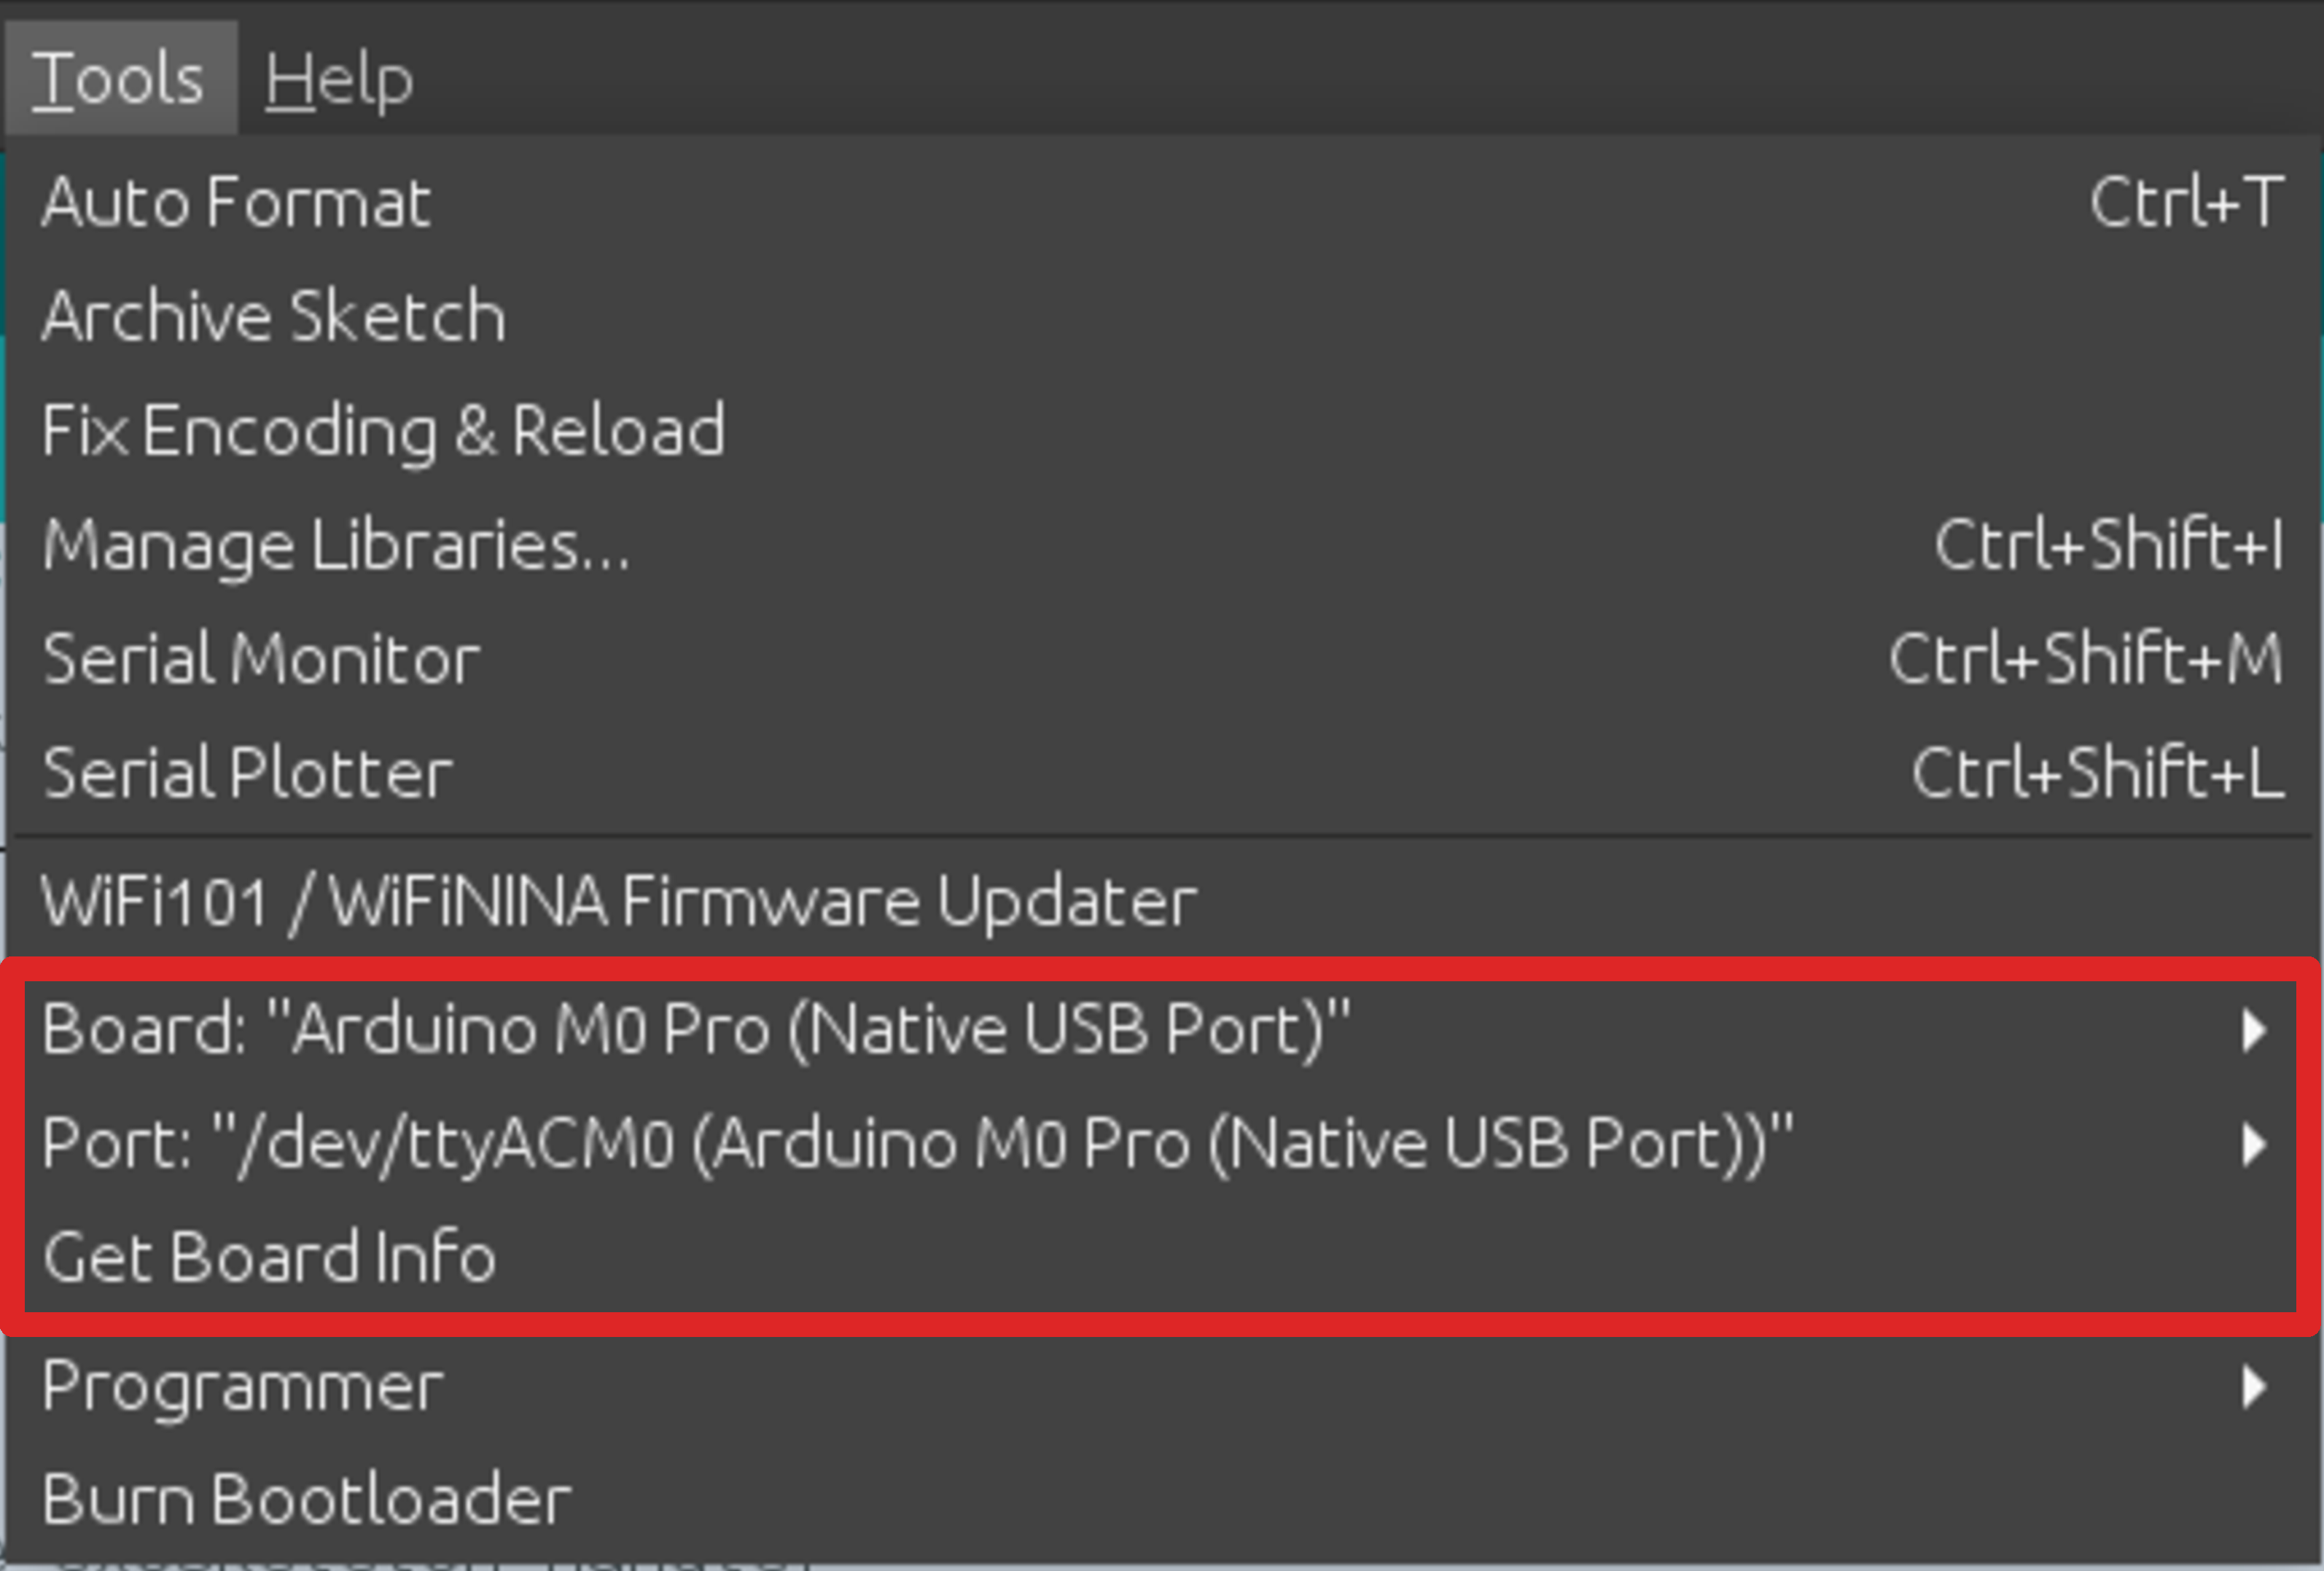
\includegraphics[width=0.45\textwidth]{Figures/arduino_setup.pdf}
        \label{fig:arduino_setup}
    }
    \qquad
    \subfloat[Arduino reset pin.]{
        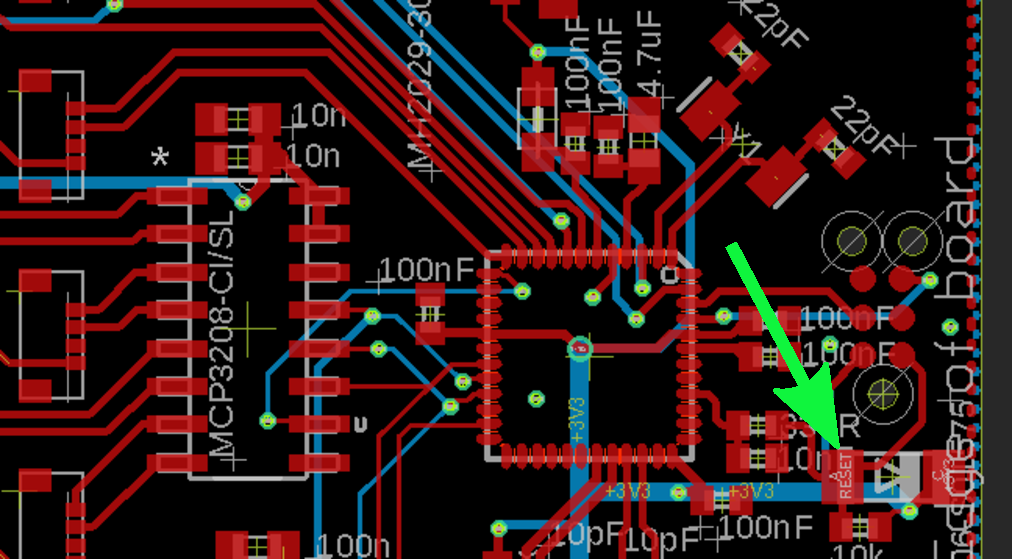
\includegraphics[width=0.45\textwidth]{Figures/reset_pin.pdf}
        \label{fig:arduino_reset_pin}
    }
    \caption{Arduino Configuration.}
\end{figure}

\subsection{Board Software}
\label{board_software}
In this project, we developed the software for the microcontroller which 
is responsible for reading the analog values produced by the 
Melexis sensors and the printing them to the serial output for further 
processing. For the source code of the software please visit 
\texttt{\href{https://github.com/amartsop/Exoskeleton}{here}},
while for the its documentation please click 
\texttt{\href{https://amartsop.github.io/Exoskeleton/index.html}{here}}.
The links also provide installation instructions.

\begin{table}
    \centering
    \begin{tabular}{ |p{2cm}||p{5cm}|p{5cm}|  }
        \hline
        \multicolumn{3}{|c|}{\textbf{Ports Mapping}} \\
        \hline
        \textit{Port ID}& \textit{Green Sensor Read Function} & \textit{Red Sensor Read Function}\\
        \hline
        $X_{1}$ & analogRead(A0) & analogRead(A1)\\
        \hline
        $X_{2}$ & analogRead(A2) & analogRead(A3)\\
        \hline
        $X_{3}$ & analogRead(A4) & analogRead(A5)\\
        \hline
        $X_{4}$ & analogRead(A6) & analogRead(A7)\\
        \hline
        $X_{5}$ & readADC(0, 4) & readADC(1, 4)\\
        \hline
        $X_{6}$ & readADC(2, 4) & readADC(3, 4)\\
        \hline
        $X_{7}$ & readADC(4, 4) & readADC(5, 4)\\
        \hline
        $X_{8}$ & readADC(6, 4) (Not Working) & readADC(7, 4)\\
        \hline
        $X_{9}$ & readADC(0, 2) & readADC(1, 2)\\
        \hline
        $X_{10}$ & readADC(2, 2) & readADC(3, 2)\\
        \hline
        $X_{11}$ & readADC(4, 2) & readADC(5, 2)\\
        \hline
        $X_{12}$ & readADC(6, 2) & readADC(7, 2)\\
        \hline
    \end{tabular}
    \caption{\label{tab:arduino_mapping}Ports mapping.}
\end{table}

Due to the daisy chaining of the sensors, each port of the board receives two
analog signals; one corresponding to the red sensor and one corresponding to the 
green sensor. Furthermore, each port can be directly connected to the 
microcontroller's built-in analog ports or it can be connected to one of the 
MCP3208 ADCs. The type of connection (direct on indirect) 
defines the way that the analog data is read by the software.
For direct connections, we can use the built-in Arduino \texttt{analogRead} 
while for indirect connection we use the custom method \texttt{readADC}.
For more information, please see the
\texttt{\href{https://amartsop.github.io/Exoskeleton/classAnalogPort.html}{AnalogPort}}
class. 
Table \ref{tab:arduino_mapping} summarizes the type of connection that 
each port allows (defined by the utilized function) as well as the wiring 
of each port (e.g. port $X_{2}$ is connected to the built-in analog ports
$A_{2}$ and $A_{3}$ of the microcontroller). The connectivity of 
the ports with the microcontroller and the ADCs was derived based on 
the \texttt{\href{https://tinyurl.com/53urrcvm}{custom PCB schematic}}.
As you can see in table \ref{tab:arduino_mapping} we only consider the 
first 12 ports, as the 13th is intended for different application.

The sensors of the exoskeleton following numbering convention shown in 
Fig. \ref{fig:sensor_numbers}. This numbering allows the mapping between 
the sensors and the board ports IDs of Fig. \ref{fig:pcb_board}.
The total number of sensors is 18, while according to our model(see 
\todo{add where to see}) the 
degrees of freedom of the exoskeleton is 13. This is 
due to the requirement of 2 extra sensors per finger for 
the measurement of the Metacarpophalangeal (MCP) angle, see 4.3.3 
in \cite{tzemanaki_anthropomorphic_nodate}. Furthermore, one degree of freedom 
(the yaw of the index finger) is ommited for simplicity.

\begin{figure}
    \centering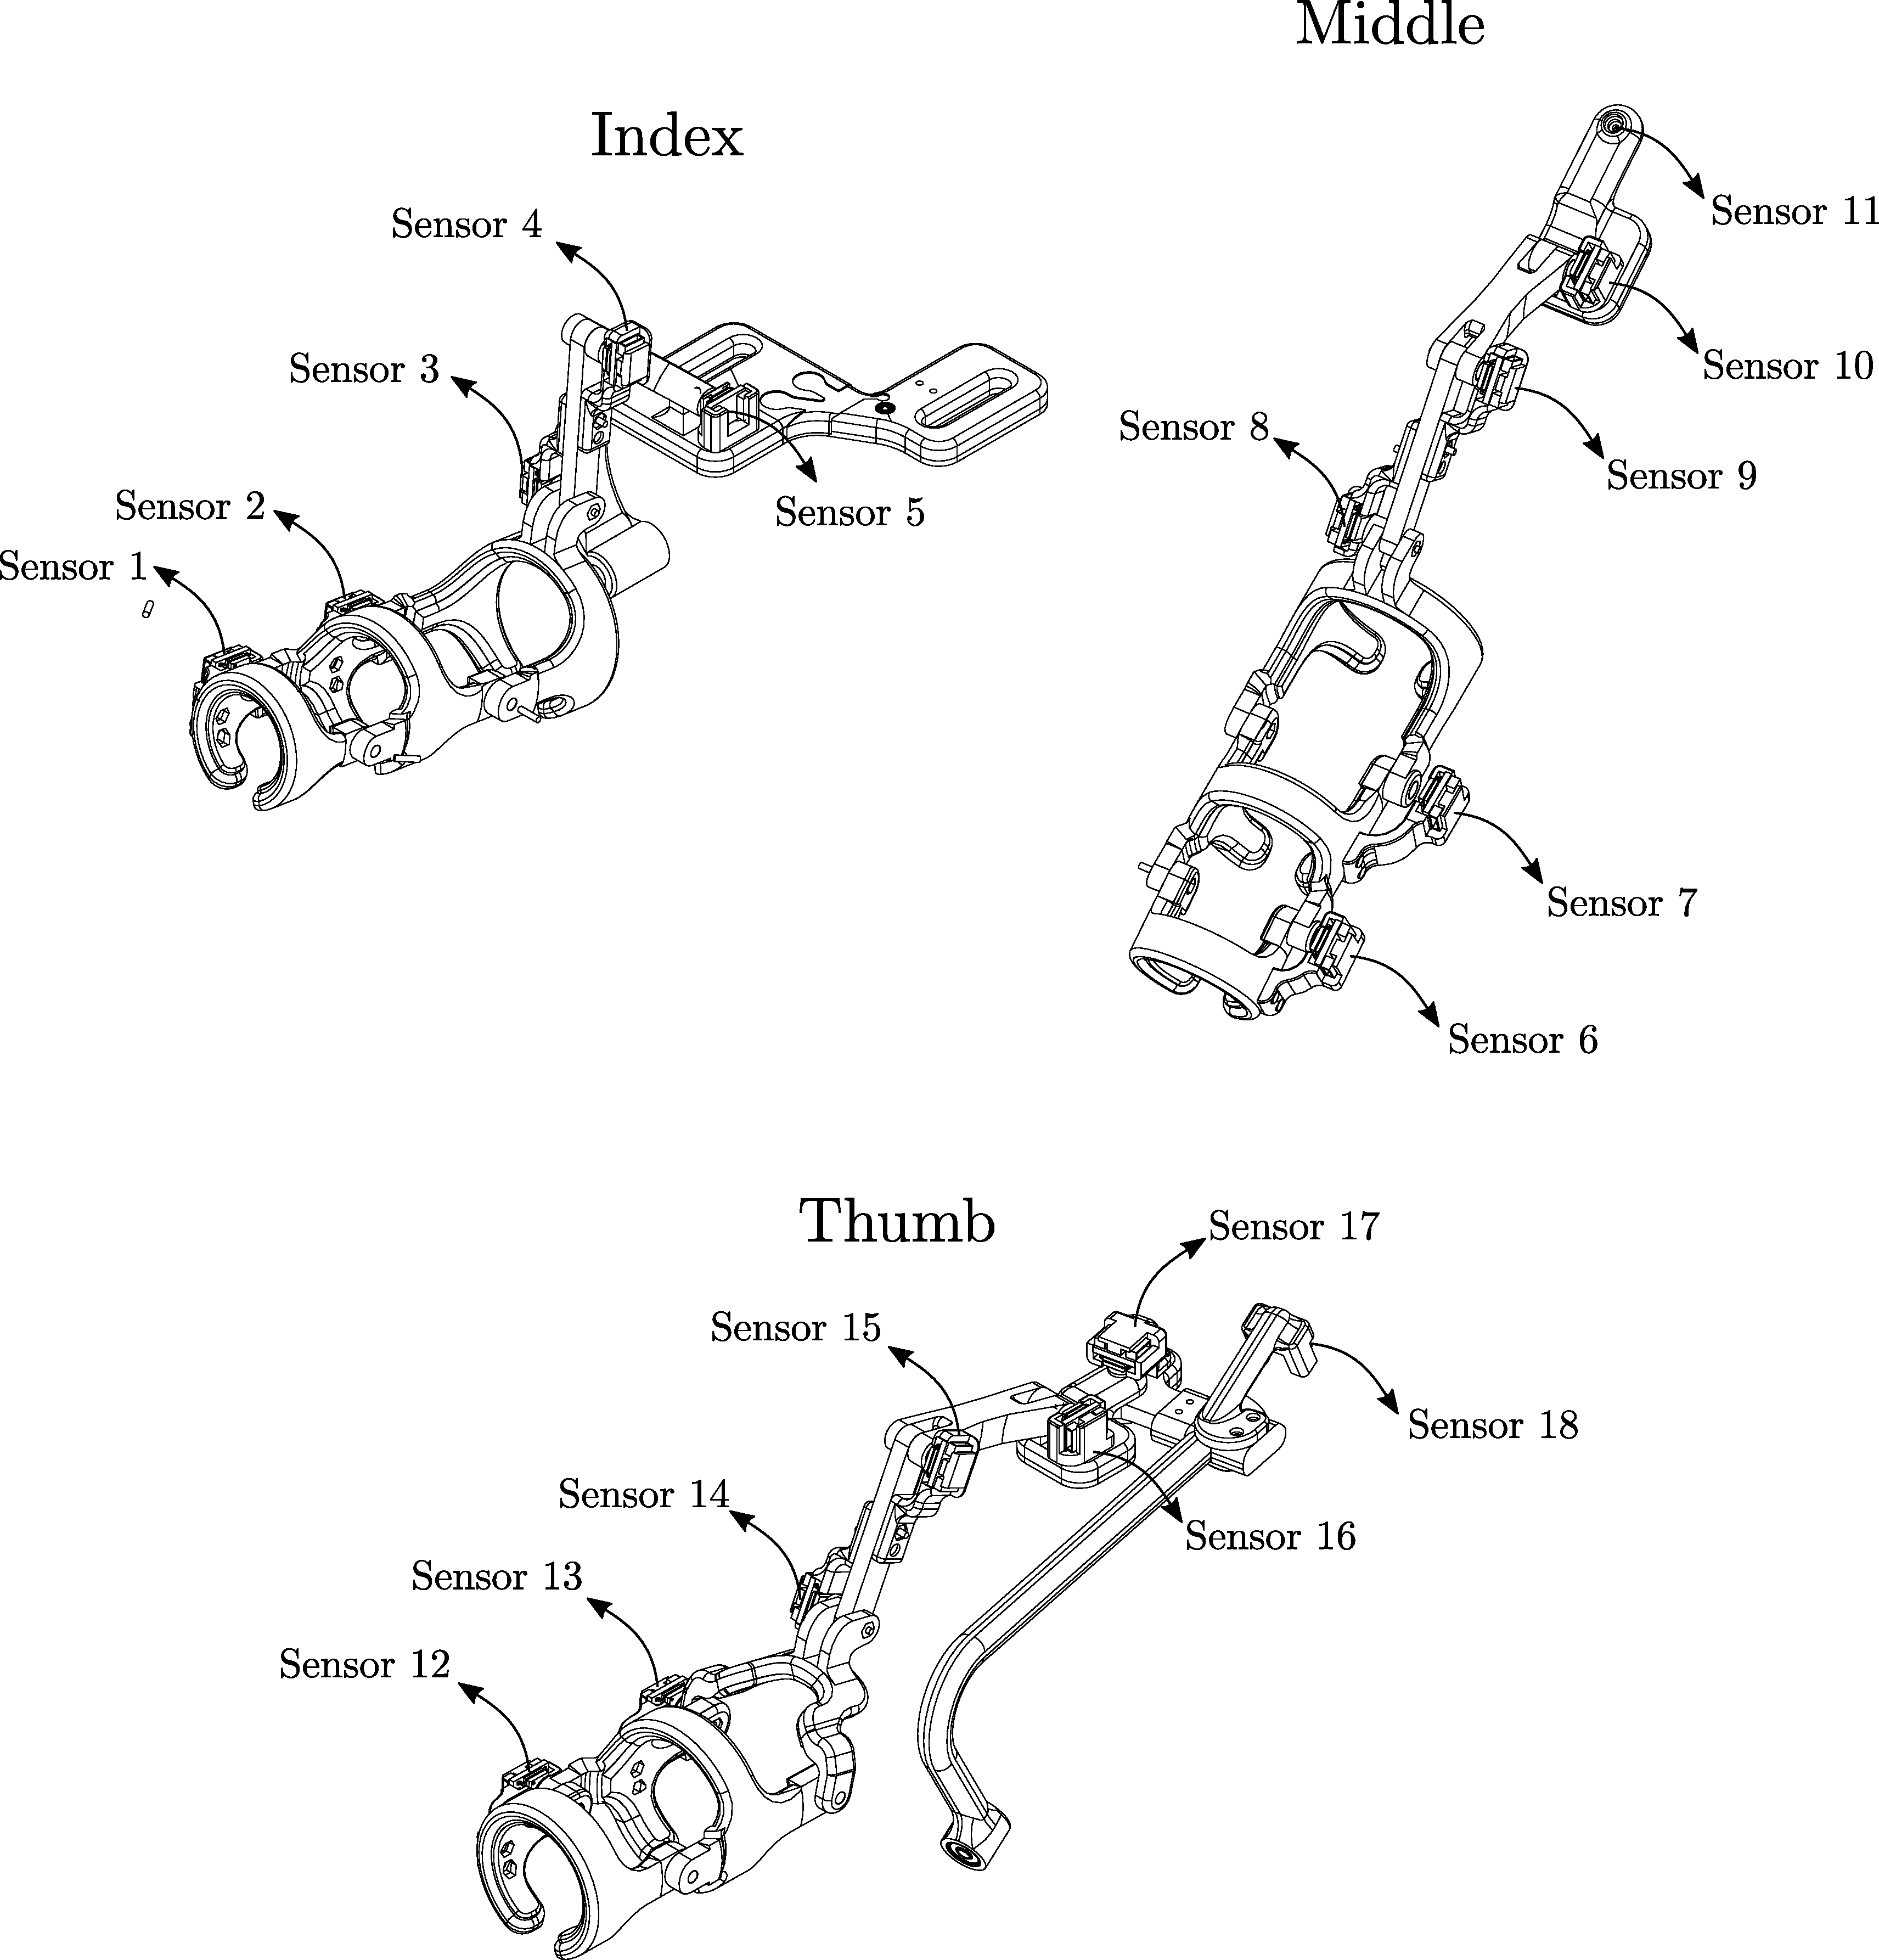
\includegraphics[width=1.0 \linewidth]{Figures/SensorNumbering.pdf}
    \caption{Custom PCB board and ports numbering convention.}
    \label{fig:sensor_numbers}
\end{figure}
Following this convention, our software gives the user the ability to connect
different sensors on different ports. This is achieved with the help of 
the initialization routine of the Sensor class.
For more information please visit 
\texttt{\href{https://amartsop.github.io/Exoskeleton/classSensor.html}{here}}.

\section{Visualisation Software}
To allow the visualization of the exoskleleton we developed two 
applications. The first, that will be referred to as \texttt{Skeletal 
Animation}, offers a photorealistic deformation of virtual hands, using the
principles of skeletal animation. The second, that will be referred to as
\texttt{Kinematic Animation}, implements a kinematically accurate
representation of the exoskeletons deformations adapted to its dimensions.
Both applications, receive the data from the exoskeleton in real-time and 
render the animation. A screen capture of both applications is
illustrated in Fig. \ref{fig:visualisation_applications}.
\begin{figure}[h]
    \centering
        \subfloat[Skeletal animation.]{
        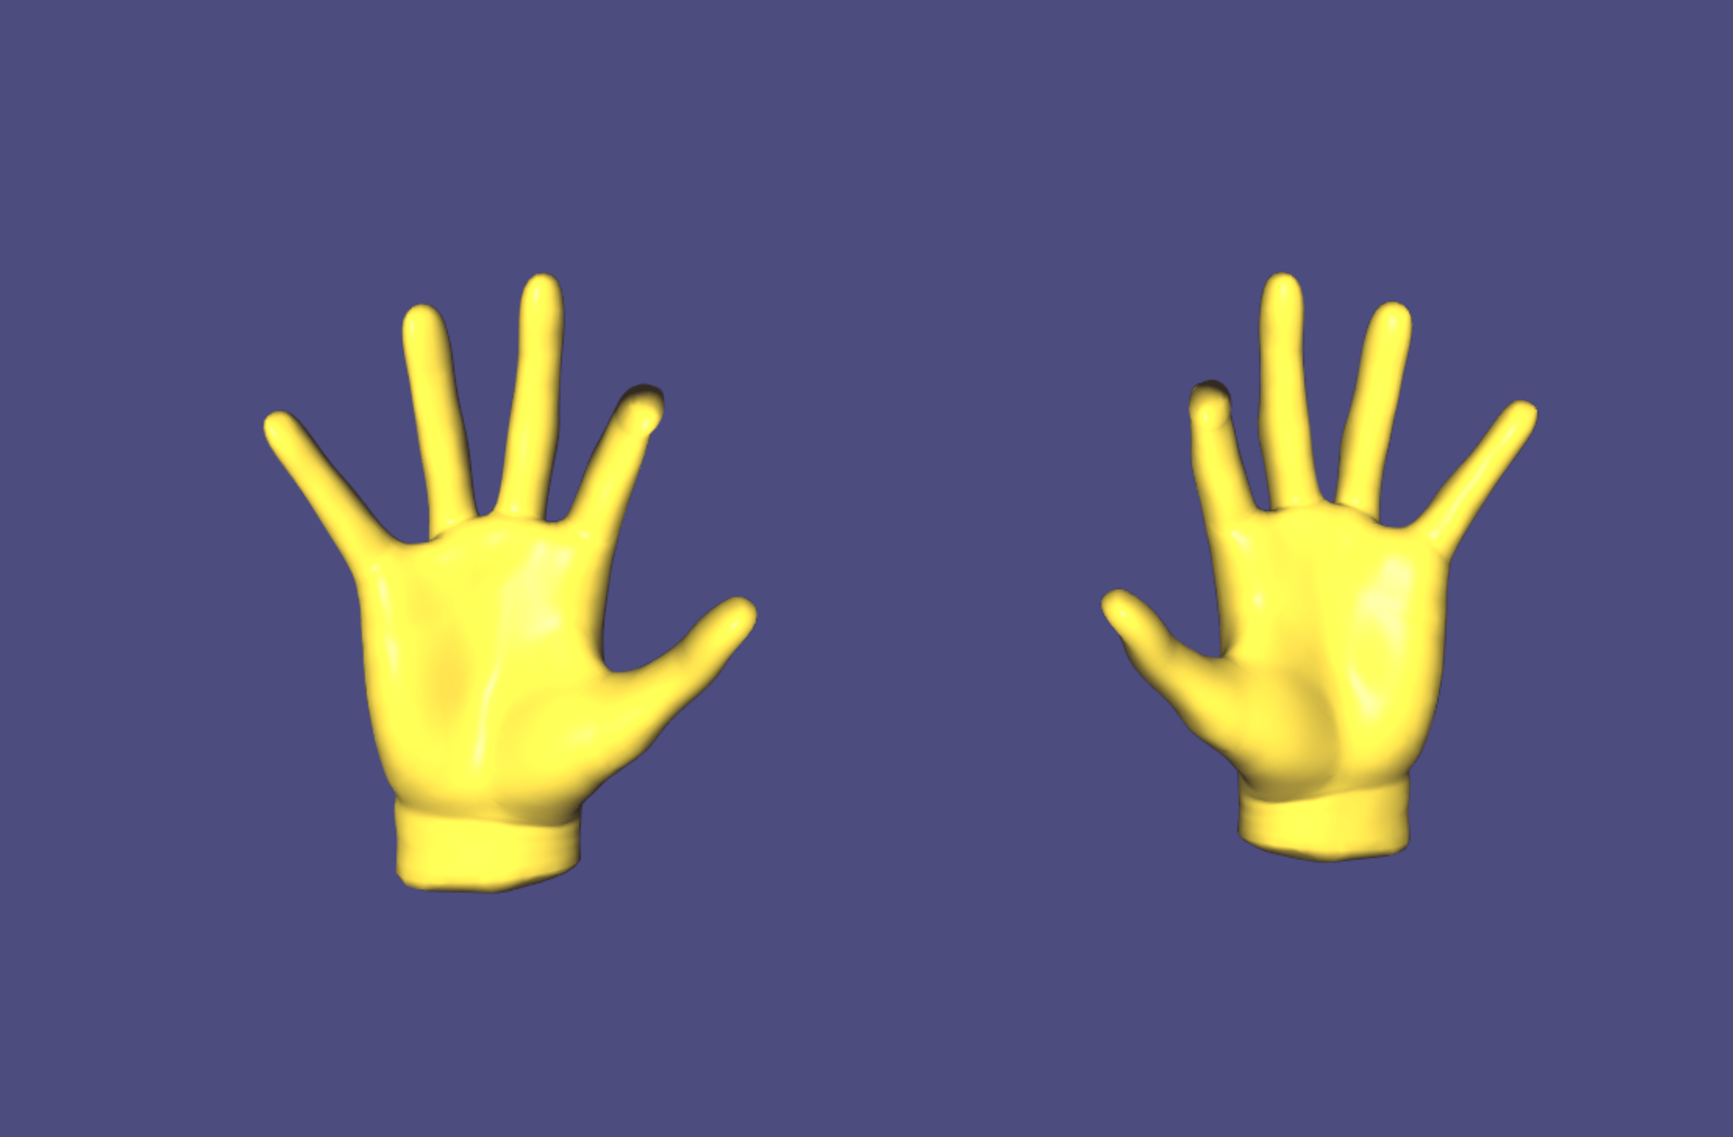
\includegraphics[width=0.45\textwidth]{Figures/animation1.pdf}
        \label{fig:animation1_capture}
    }
    \qquad
    \subfloat[Kinematics animation.]{
        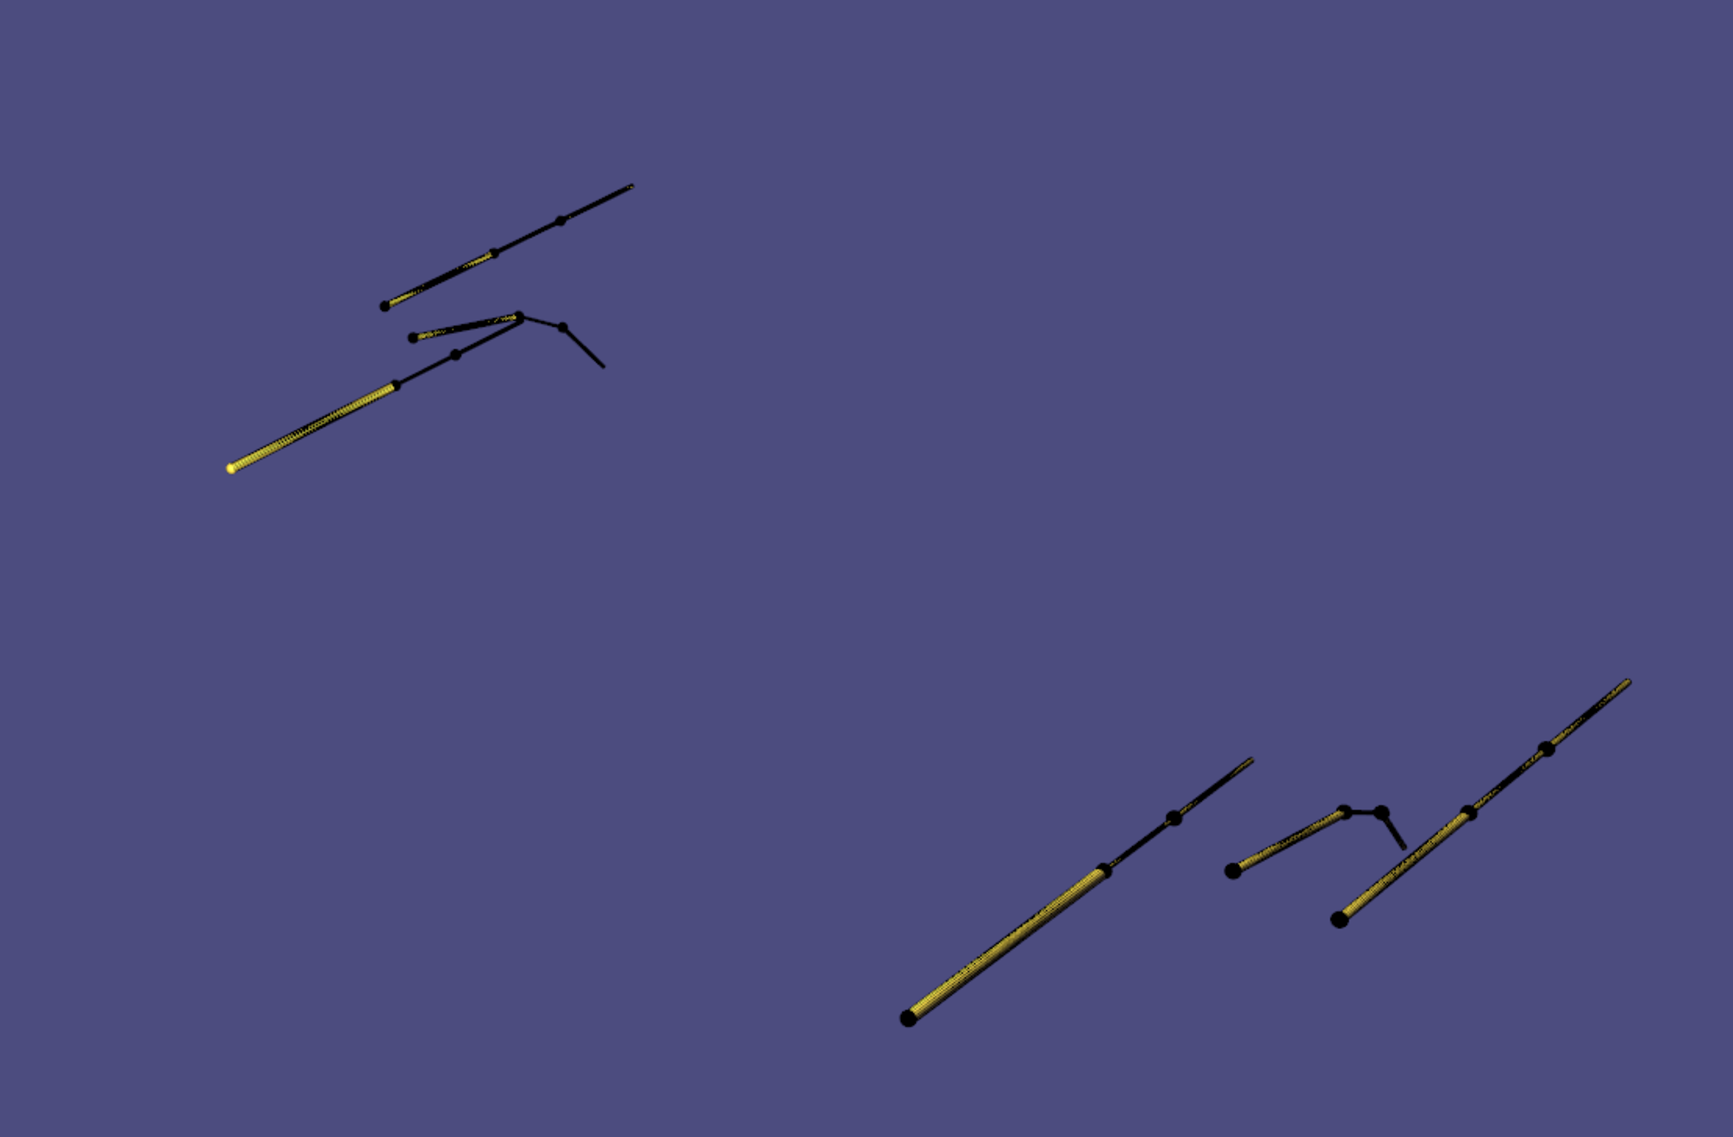
\includegraphics[width=0.45\textwidth]{Figures/animation2.pdf}
        \label{fig:animation2_capture}
    }
    \caption{The two visualisation applications.}
    \label{fig:visualisation_applications}
\end{figure}
Furthermore, our applications can capture real-time video stream and 
perform face landmarking with the help of Google's machine learning library 
\texttt{\href{https://google.github.io/mediapipe/solutions/face_mesh.html}{MediaPipe}}.
The data are then sent in real-time to the animation environment and they 
get rendered. A screen capture of the face landmarking application, that 
will be reffered to as \texttt{Skeletal Animation Face}, is illustrated
in Fig. \ref{fig:hands_face}. 
\begin{figure}[h]
    \centering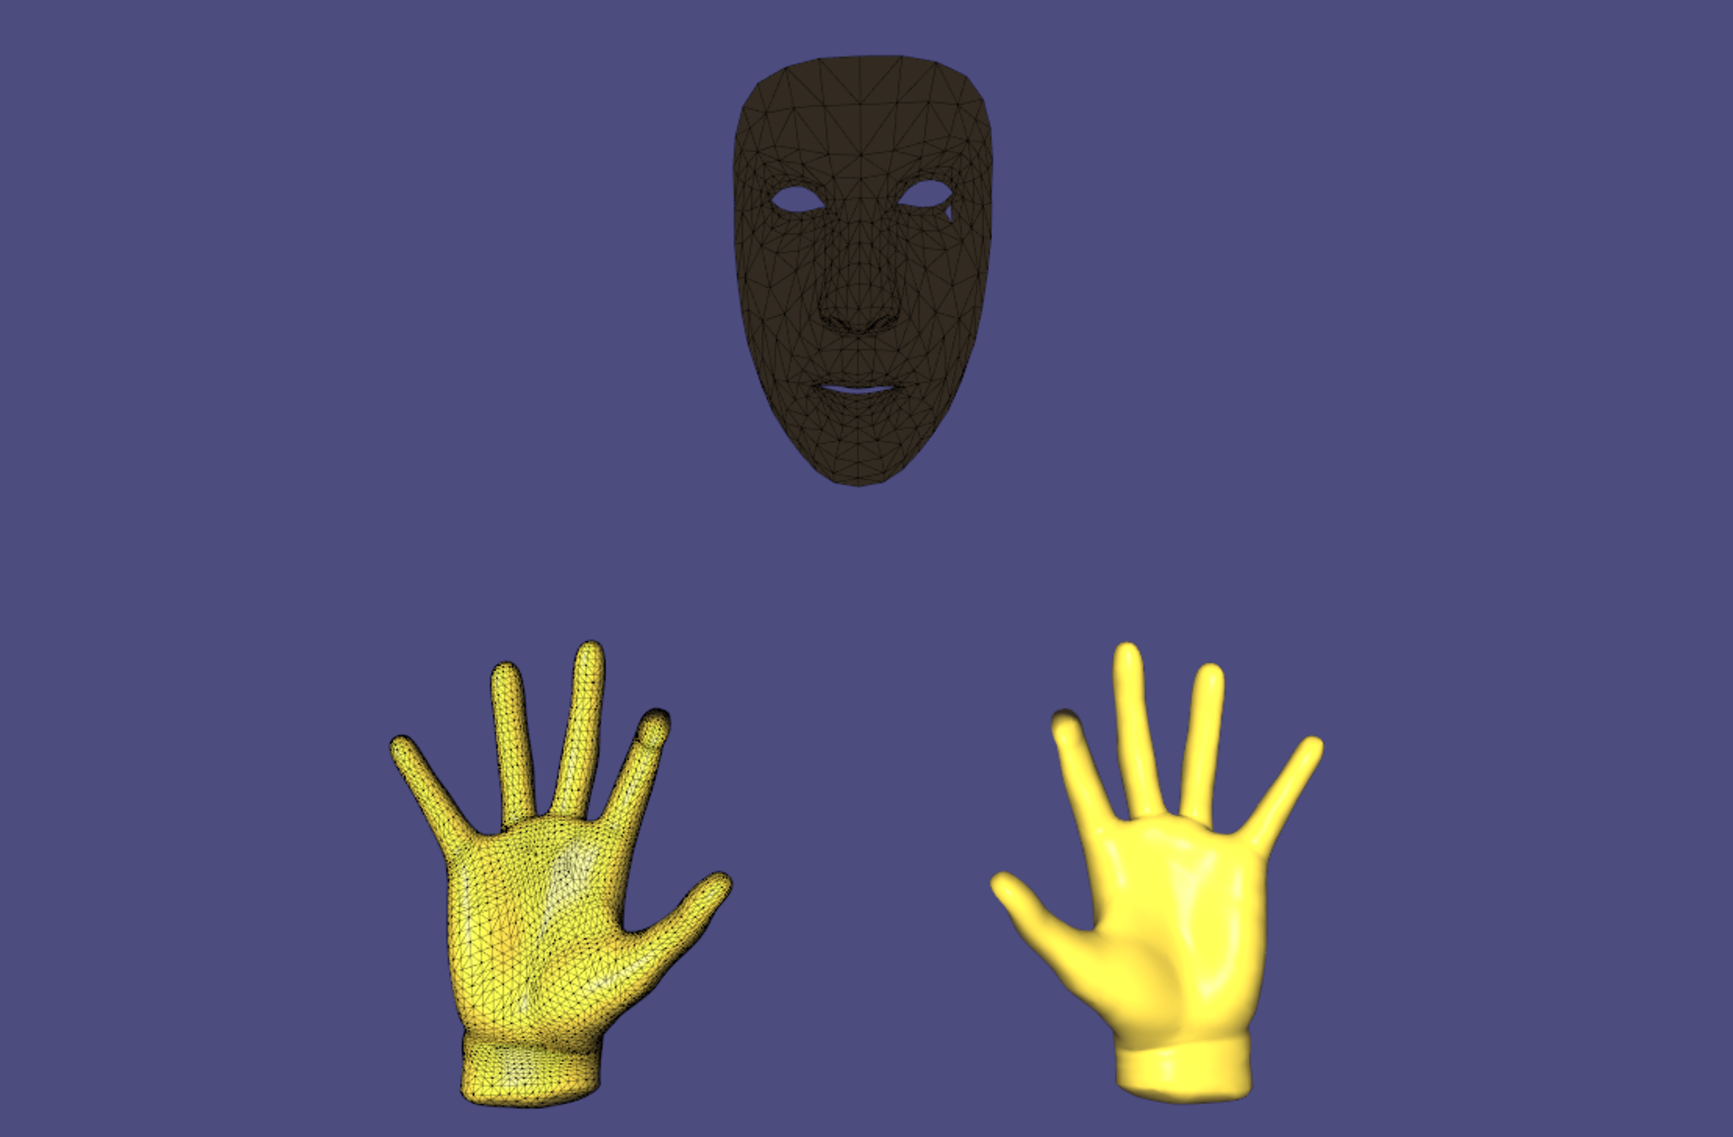
\includegraphics[width=0.8 \linewidth]{Figures/hands_face.pdf}
    \caption{Hands and face rendering.}
    \label{fig:hands_face}
\end{figure}
\subsection{Core Libraries}
Our software depends on two key liraries; the
\texttt{\href{https://libigl.github.io/tutorial/}{LibIGL}} lirary and 
the
\texttt{\href{https://google.github.io/mediapipe/solutions/face_mesh.html}{MediaPipe}}
library.

\subsubsection{LibIGL}
LibIGL is an open source C++ library for geometry processing research
and development. LibIGL builds on top of OpenGL and its
API gives a high level control of geoemrtry rendering 
without the need for low level manipulation of graphics primitives, such as 
fragment and geometry shaders. The library uses 
\texttt{\href{https://eigen.tuxfamily.org/index.php?title=Main_Page}{Eigen}}
to encode vectos and mutrices. A triangular mesh is encoded as pair of 
matrices:
\begin{verbatim}
    Eigen::MatrixXd V; 
    Eigen::MatrixXd F;
\end{verbatim}
where $V$ is a $n \times 3$ matrix which stores the coordinates of the vertices,
with $n$ the number of vertices in the geometry. Each row stores the 
coordinates of a vertiex, with its $x, y$ and $z$ coordinates in teh first, 
second and third column, respectively. The matrix $F$ stores the triangle 
connectivity: each line of $F$ denotes a trinagle whose 3 vertices are 
represented as indices pointing to rows of $V$. Fig. \ref{fig:simple_mesh}
shows a representation of a simple mesh using the storage mechanism of 
LibIGL.
\begin{figure}
    \centering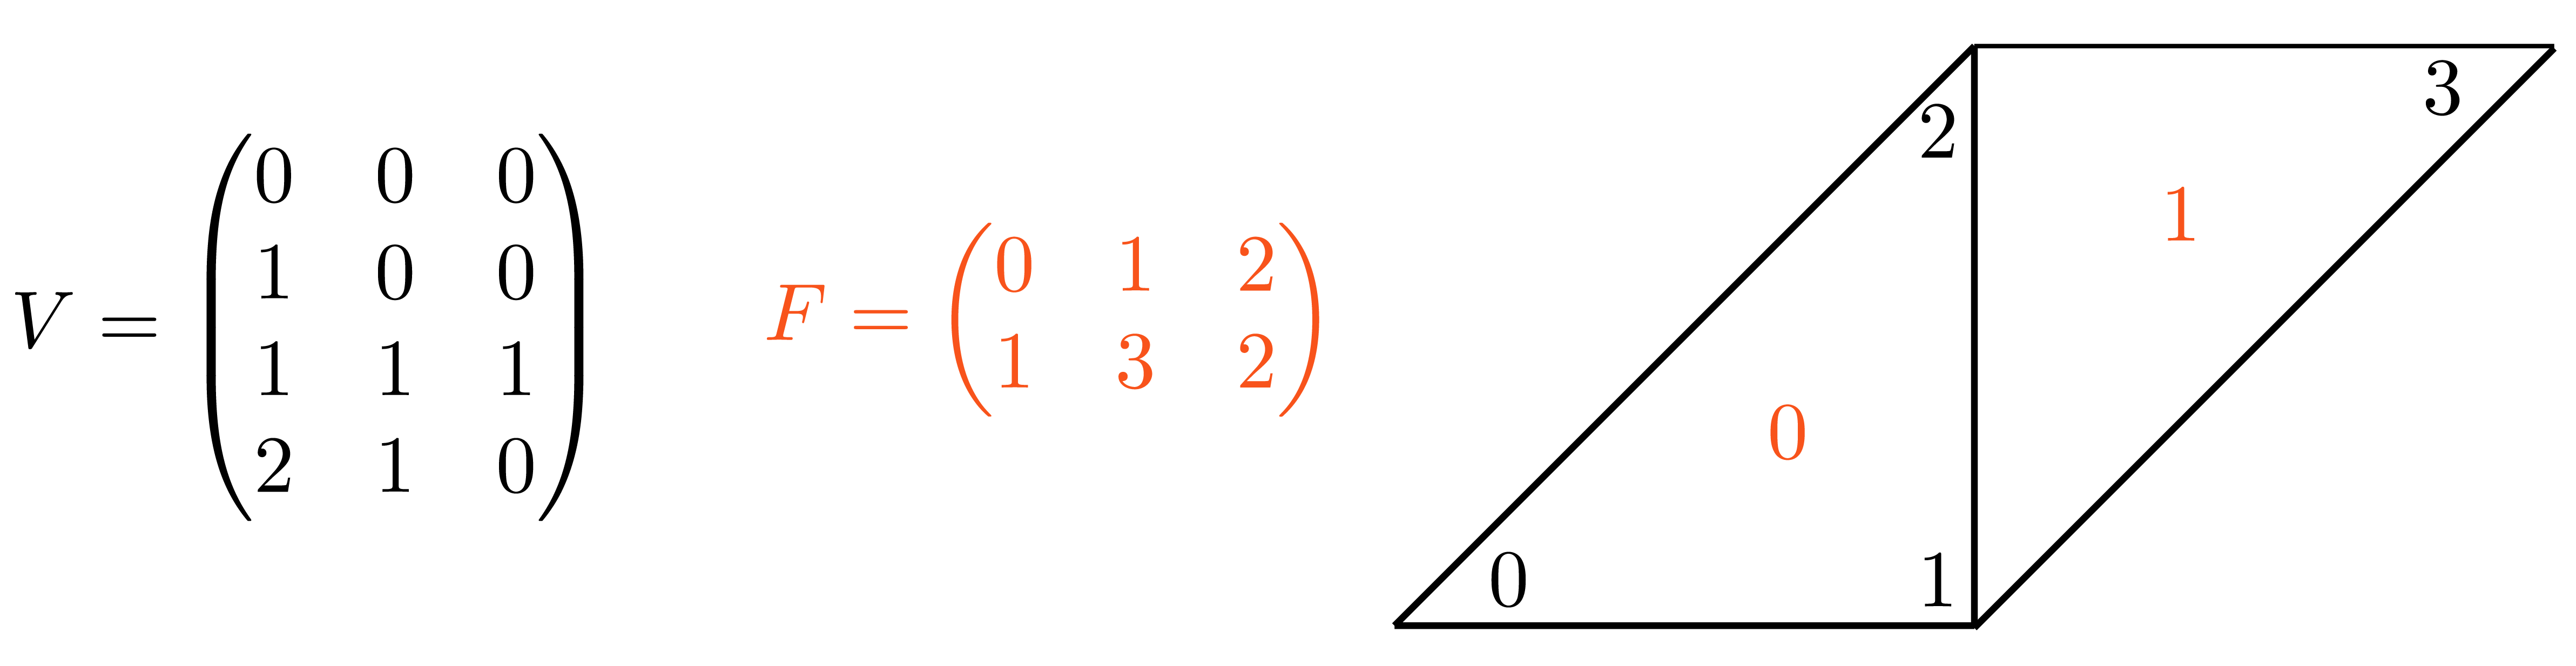
\includegraphics[width=1.0 \linewidth]{Figures/libigl_vf.png}
    \caption{LibIGL representation of a simple mesh made of 2 triangles and 4
    vertices.}
    \label{fig:simple_mesh}
\end{figure}
Note that the order of the vertex indices in $F$ determines the orientation
of the triangles and it should thus be consistent for the entire surface. 
For more information about the library please visit
\texttt{\href{https://libigl.github.io/tutorial/}{LibIGL}}.

\subsubsection{MediaPipe}
MediaPipe Face Mesh is a face geometry solution that estimates 468
3D face landmarks in real-time, as shown in \ref{fig:mediapipe_mesh}. It
employs machine learning (ML) to infer the 3D surface geometry, requiring only a
single camera input without the need for a dedicated depth sensor. Utilizing
lightweight model architectures together with GPU acceleration throughout
the pipeline, the solution delivers real-time performance critical for
live experiences. The library is combined with our rendering application 
to allow real-time rendering of a face mesh, using just a webcam. To run the 
library we use the Python API combined with OpenCV for image acquisition.
The user can find the Python script 
\texttt{\href{https://github.com/amartsop/SkeletalAnimationMultiThreadFace/blob/master/face_mesh_server.py}{here}},
while for more information on MediaPipe please visit 
\texttt{\href{https://google.github.io/mediapipe/solutions/face_mesh.html}{here}}.
\begin{figure}
    \centering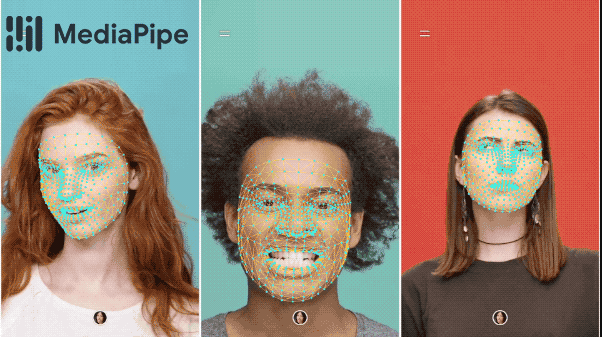
\includegraphics[width=1.0 \linewidth]{Figures/mediapie.png}
    \caption{MediaPipe mesh.}
    \label{fig:mediapipe_mesh}
\end{figure}

\subsection{Dependencies and Installation}

\subsubsection{LibIGL Dependencies}
Our software has some core dependencies that need 
to be installed before use. As we discussed before, the core dependency of
LibIGL are the Eigen C++ linear algebra library. Our software also uses
the GLFW library creating windows, contexts and
surfaces, receiving input and events and the dear ImGui for 
the graphical user interface. Installation of LibIGL and its dependicies 
is done with the help of the \texttt{\href{https://cmake.org/}{CMake}} build
system. LibIGL can be installed as a header-only library or as a static 
library. Installing as a static library leads to significantly less 
compilation time. In this regard, our software builds the static version of 
the library. However, as discussed \texttt{\href{https://libigl.github.io/static-library/}{here}}
in the case of static compilation special care must be taken by the developers
of each function and class in the LibIGL library that uses C++ templates. 
Analyical instructions for avoiding compilation errors for templated functions
are presented \texttt{\href{https://libigl.github.io/static-library/}{here}}.
In the case that the user prefers a header-only installation of LibIGL
and of our software this is provided here. \todo{add repo}
In the case the user wants to further develop our software, a full list of 
LibIGL dependencies is given 
\texttt{\href{https://libigl.github.io/third-party/}{here}}.

\subsubsection{MediaPipe Dependencies}
For our application the MediaPipe library is combined with \texttt{OpenCV} for 
real-time image acquisition and the \texttt{numpy} module for linear 
algebra operations. For the installation of the library see
\ref{installation}.

\subsubsection{Other Dependencies}
As discussed before, our software allows the user to combine MediaPipe and 
LibIGL and render face-landmarking data in real time. Since the LibIGL 
is a C++ application and MediaPipe is a Python application an 
\href{https://en.wikipedia.org/wiki/Inter-process_communication}{inter-process}
communication between the two is recquired. For this, we use C++ and 
Python sockets, to establish a TCP communication between the two applications.
The data is transmitted between the two applications with the help 
of the \texttt{\href{https://www.json.org/json-en.html}{JSON}} data-interchange 
format. To allow the generation and parsing of JSON files we use 
\texttt{\href{https://docs.python.org/3/library/json.html}{JSON module}} on the 
Python side and the header-only
\texttt{\href{https://github.com/nlohmann/json}{nlohmann-json}} library on the
C++ side. Further dependencies can be found in the provided
\texttt{\href{https://github.com/amartsop/SkeletalAnimationMultiThreadFace/blob/master/.installation.sh}{.installlation.sh}}
script.

\subsubsection{Installation}
\label{installation}
As discussed before, the software has multiple dependencies. To fascilitate 
the installation process we have created a shell script document that 
automatically installs all the required dependencies. The current version of 
the software runs only in Linux, but extension to Windows platforms is also 
possible. The installation process for all the three provided applications
(Skeletal Animation", Kinematic Animation and Skeletal Animation Face)
is the same. The steps for installing the appropriate software
are the following:

\begin{itemize}
    \item Clone the appropriate github repository to your local directory.
    \begin{lstlisting}{bash}
        $git clone https://github.com/amartsop/Project.git 
    \end{lstlisting}
    \noindent where "Project" can be one of the following:
    \begin{itemize}
        \item SkeletalAnimationMultiThread,
        \item KinematicsAnimationMultiThread,
        \item SkeletalAnimationMultiThreadFace.
    \end{itemize}
    
    \item Install the appropriate dependencies. This can be done manually 
    or with the help of the inculded installation bash script 
    \texttt{ \href{https://github.com/amartsop/SkeletalAnimationMultiThreadFace/blob/master/.installation.sh}{.installlation.sh}}.
    If the user wants to install dependencies manually, the full list 
    of them is included in the provided \texttt{ \href{https://github.com/amartsop/SkeletalAnimationMultiThreadFace/blob/master/.installation.sh}{.installlation.sh}}
    file. To execute the installation file:
    \begin{enumerate}
        \item Login as root and navigate to the directory where the installation 
        file is located.
        \item Run 
    \begin{lstlisting}{bash}
        $source ./.installation.sh
    \end{lstlisting}
    \noindent \textbf{Warning}: This will install quite a few libraries and 
    packages in your computer. Please make sure that you are aware of the 
    packages that are installed and with the location in which they are installed.
    Both settings can be changed by editing the ".installations.sh" file.
    \end{enumerate}

    \item Build the provided software. To do this:
    \begin{enumerate}
        \item Navigate to the home location of the directory you have cloned. 
        \item Generate a build directory and navigate to it by executing:
            \begin{lstlisting}{bash}
                $mkdir build && cd build
            \end{lstlisting}
        \item Execute the CMake file by running:
        \begin{lstlisting}{bash}
            $cmake ..
        \end{lstlisting}
        \item Build the executable by running:
        \begin{lstlisting}{bash}
            $make -j4
        \end{lstlisting}
        \noindent \textbf{Note}: Using the command "-j4" we ask the compiler 
        to use 4 threads for build the executable. The user can use as many as 
        they prefer. The first time that you build the executable, LibIGL fetches 
        its files from github and builds them as a static library. Since LigIGL 
        is a quite heavy library this will take a while. However, all the 
        following build commands will not build the LibIGL again but only the 
        files that the user has added. If you want to update your build directory 
        we recommend deleting the "CMakeCache.txt" file in it instead of deleting 
        the whole build directory (as this will mean that the user will have To
        build LibIGL from scratch).
    \end{enumerate}
    
\end{itemize}

\subsubsection{Other Considerations}
The applications that we developed need to process data simulataneously from 
multiple source. More specifically, our applications need to read in real-time
serial-data from two sources (for the two hands), acquire image 
data from the camera, process everything and render them on the screen. 
Furthermore, the frequency of these different processes varies significantly 
among them. For example the seria data acquisition process is significantly 
faster than the rendering process. In this regard, handling 
all these operations using a single recursive loop is not fisibile, not 
only because of the variability of frequencies but also because such an 
approach would create significant lag between the data acquisition and rendering.
To tackle this problem, we recognize that the acquisition of the data for 
the different processes can be performed concurently (the processes are decoupled).
In this regard, our software splits the different tasks in seperate threads. 
Each thread is respsonsible for capturing incoming data recusrsively
and when all the thread are finished the final results is rendered on the
screen. Threading in our applications is performed with the help of the 
C++ standard library and more specifically the
\href{https://en.cppreference.com/w/cpp/thread/async}{async function}.
Except for multithreading, we have also used forking for process creation
\texttt{\href{https://github.com/amartsop/SkeletalAnimationMultiThreadFace/blob/master/main.cpp}{here}}.
For more on forking please visit 
\texttt{\href{https://man7.org/linux/man-pages/man2/fork.2.html}{here}}.

It should be noted that \todo{add ros part}

\subsection{Kinematic model}
In this section we discuss some of aspects of the 
proposed kinematic hand/exoskleton model. This model
allows the mapping the exoskeleton movement to the movenemt of a
virtual hands. In our model only three fingers are studied; namely the 
thumb, the index and the middle finger. In Fig. \ref{fig:kinematic_model}
we represent the kinematic model that we use as the basis for modeling the
exoskeleton's movement (left hand). 
\begin{figure}
    \centering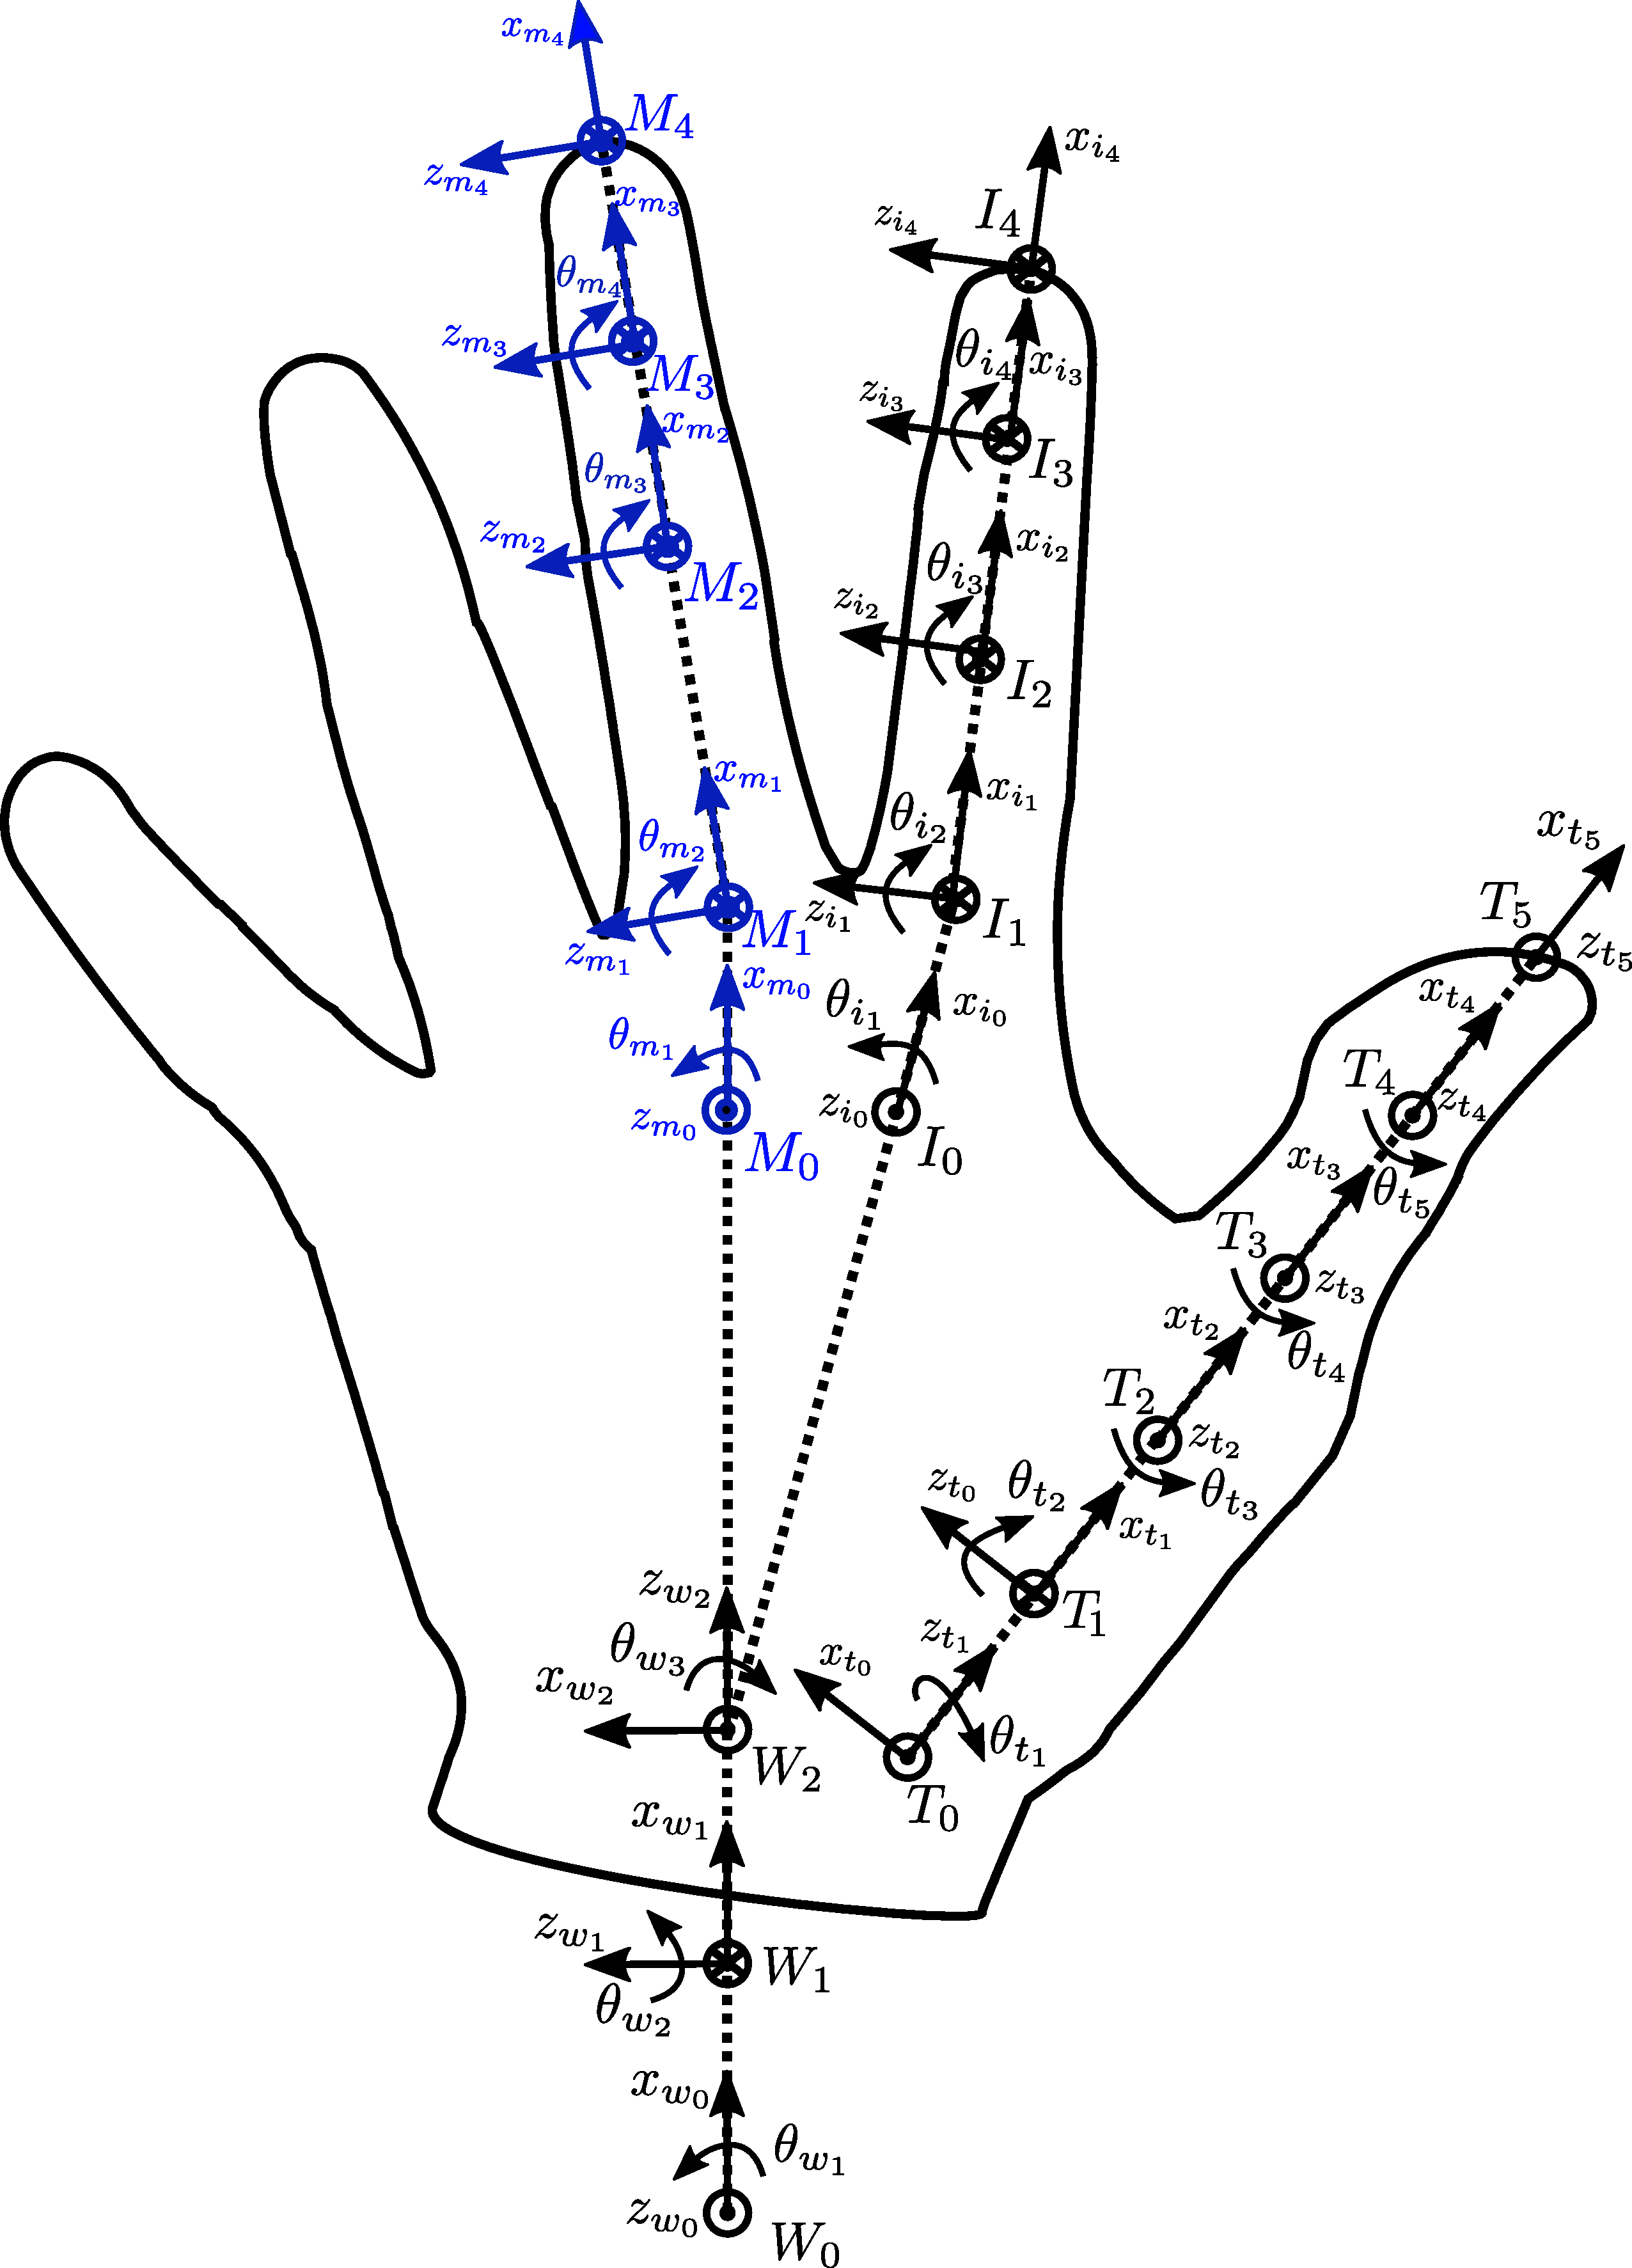
\includegraphics[width=0.8 \linewidth]{Figures/kinematic_model.pdf}
    \caption{Kinematic model of left hand.}
    \label{fig:kinematic_model}
\end{figure}
The joint angles measured from the exoskeletons are directly mapped to this 
model. For example, the angle measured from sensor 1 in Fig. \ref{fig:sensor_numbers}
corresponds to the angle $\theta_{i_{4}}$ of Fig. \ref{fig:kinematic_model}.
It should be noted that the angles $\theta_{w_1}, \theta_{w_2}$ and 
$\theta_{w_3}$ are not used by can be easily incorporated into the current model.
It is important to note that this kinematic model is
decoupled from the animation used. As we will discuss below, the avatars 
that will be introduced to represent the virtual hands can have their own 
frame conventions. However, all avatars must report to the basis frame 
convention shown in Fig. \ref{fig:kinematic_model} as this is the one 
corresponding to the actual motion of the physical exoskeleton. The mapping 
between the avatar frames and the basis frame convention is discussed 
in the following paragraphs. 

\subsection{Kinematic Animation}
This application allows for a kinematically accurate representation of the 
hands movement. Each finger is represented by a set of cylinders that represent 
the finger's phalanges and a set of spheres representing the finger's 
knuckles. The lengths of the phalanges and knuckes are determined based on 
the configuration file that correspond to the specific dimensions of the 
exoskeleton (see file \texttt{\href{https://github.com/amartsop/KinematicsAnimationMultiThread/blob/master/share/hand_config.json}{here}}).
To allow the accurate representation of the hand's forward kinematics, the 
user can edit the configuration file based on their exoskeleton measurements.

The virtual hand follows the frame convention shown in Fig. \ref{fig:kinematic_animation_model}.
As shown in Fig.\ref{fig:model_comparison_kinematic_animation} the 
frames of the kinematic animation differ from the original/basis frame 
convention. However, mapping the configuration of the original kinematic model 
to that of the virtual hand is straightforward. The process is analytically
documented 
\texttt{\href{https://amartsop.github.io/KinematicsAnimationMultiThread/classAnimatedHand.html}{here}}.
The source code of the project can be found 
\texttt{\href{https://github.com/amartsop/KinematicsAnimationMultiThread}{here}}
while the full documentation of the application is
\texttt{\href{https://amartsop.github.io/KinematicsAnimationMultiThread/index.html}{here}}.

In Fig. \ref{fig:animation2_capture} we present the rendering result of 
the \texttt{Kinematic Animation Model}.
\begin{figure}[h]
    \centering
        \subfloat[Original kinematic model.]{
        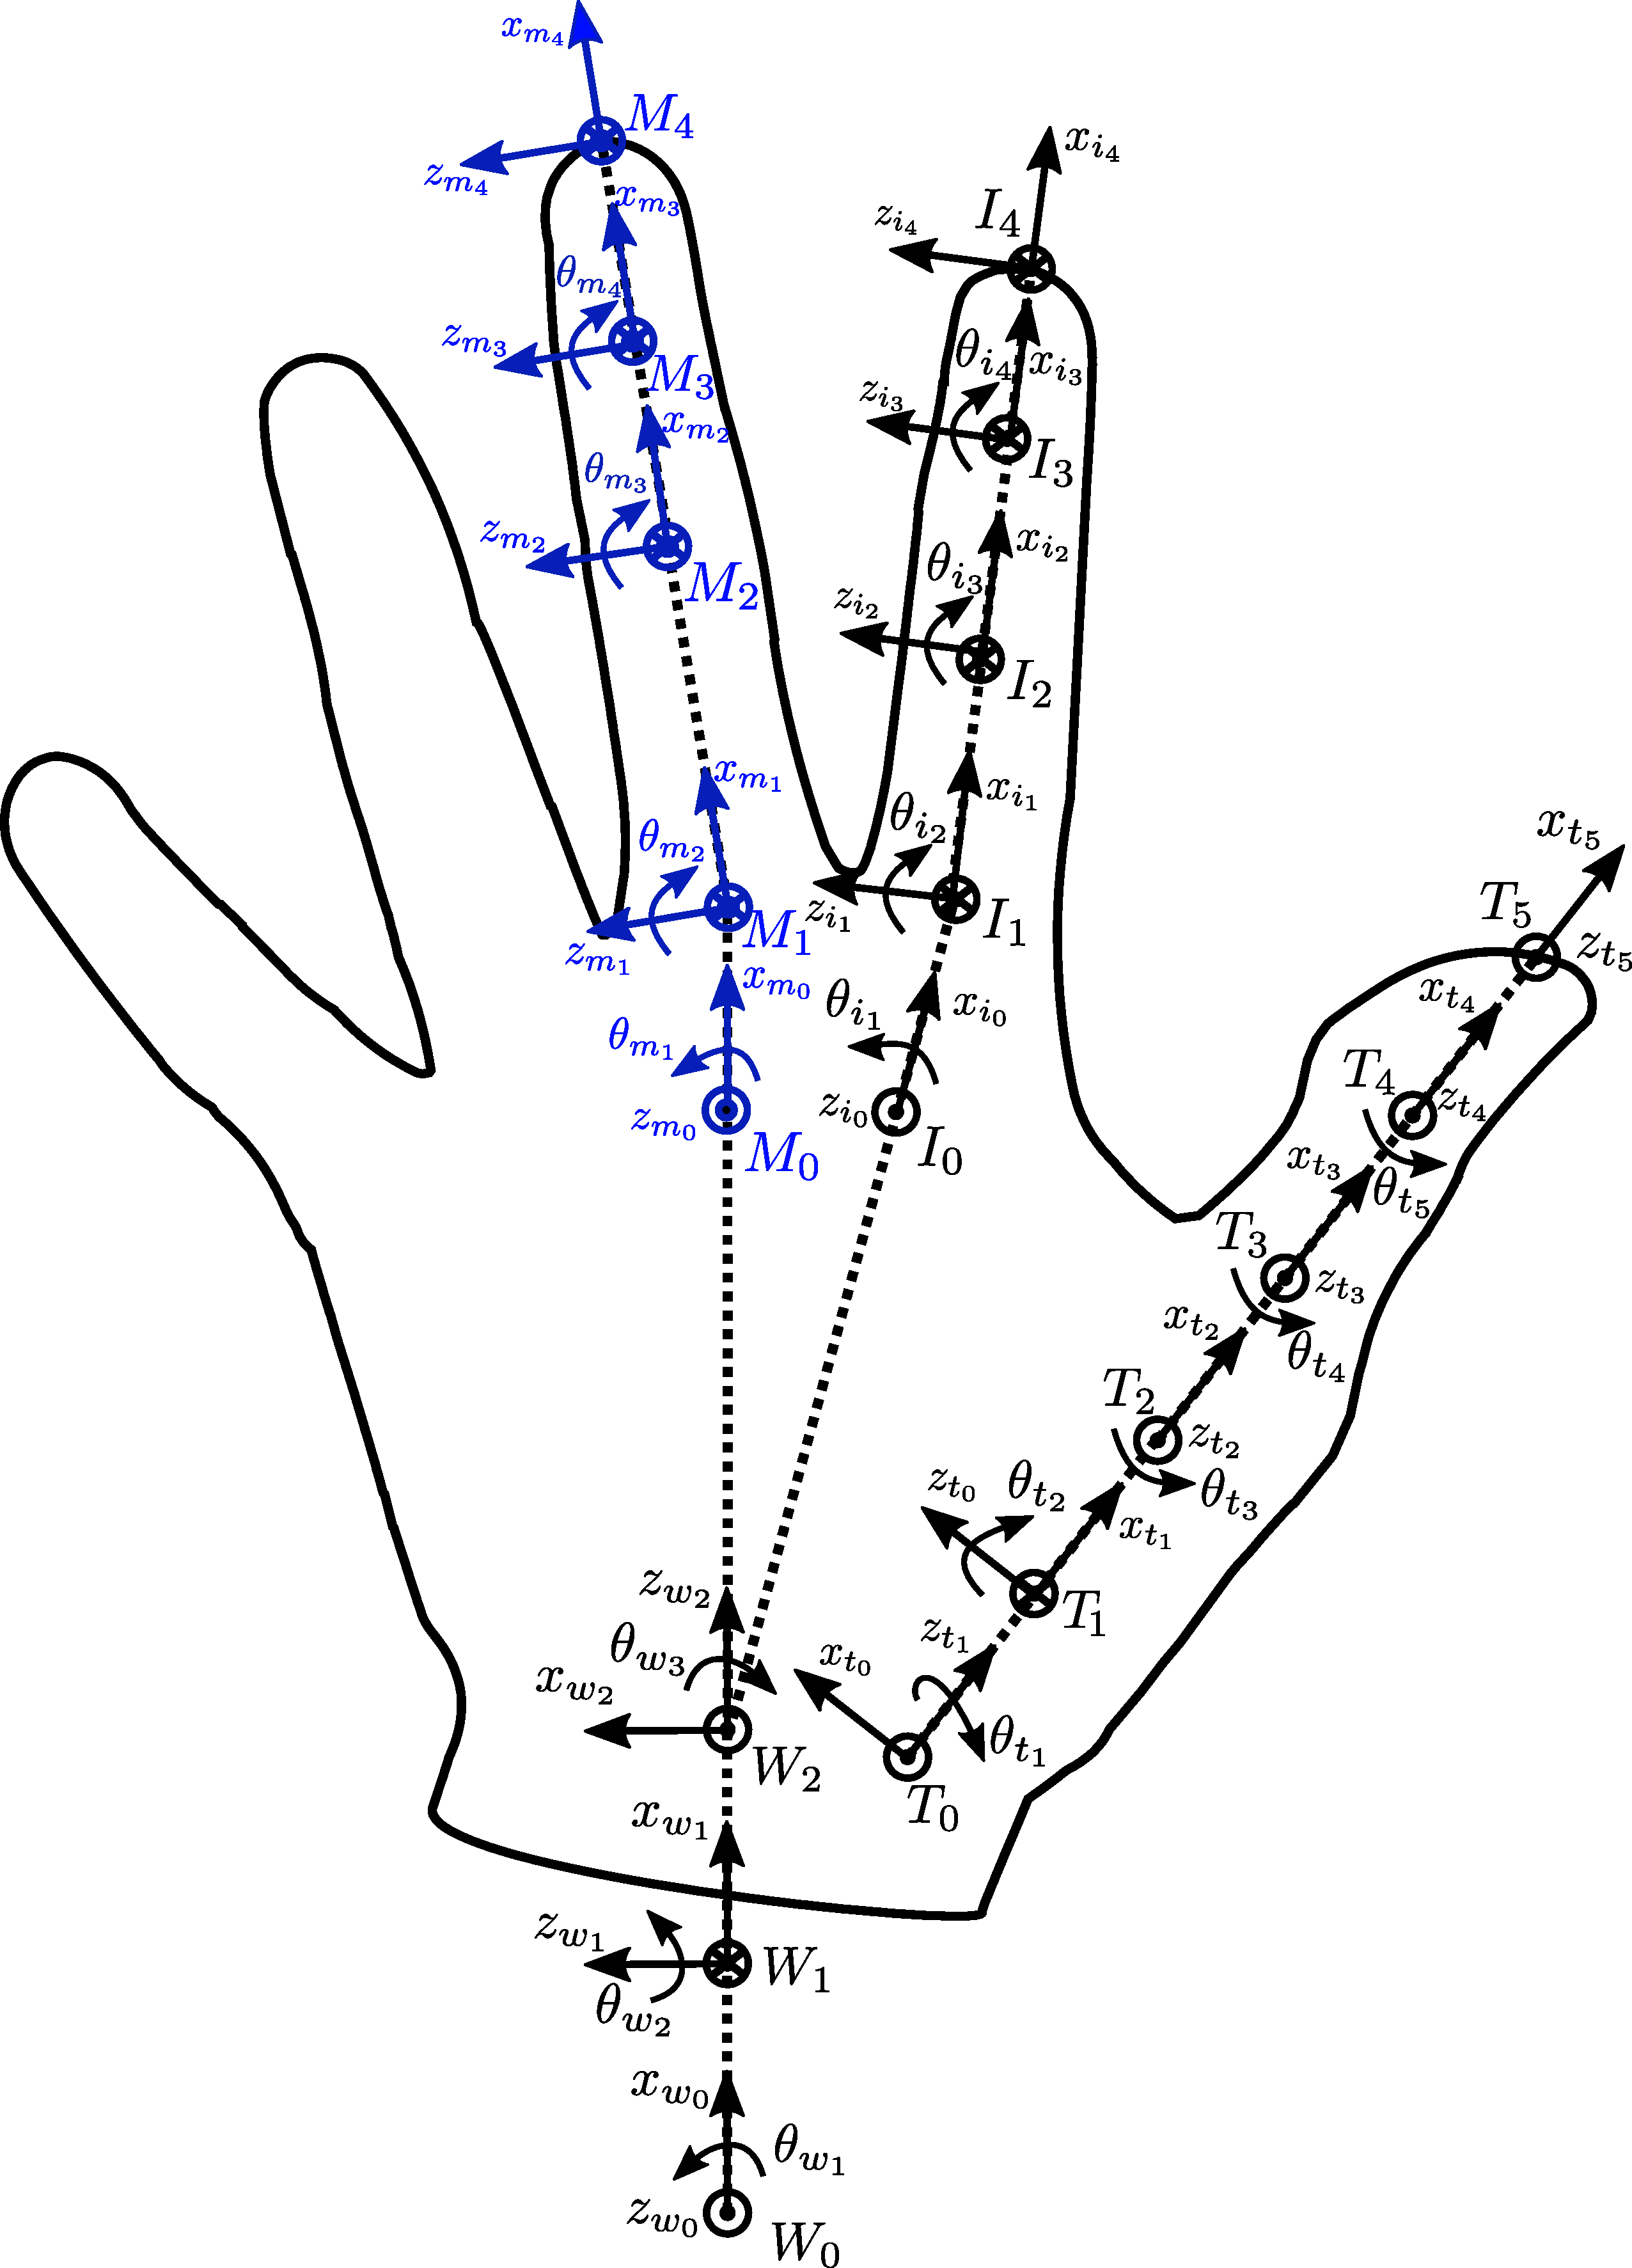
\includegraphics[width=0.45\textwidth]{Figures/kinematic_model.pdf}
        \label{fig:kinematic_model_comparison}
    }
    \qquad
    \subfloat[Animation kinematic model.]{
        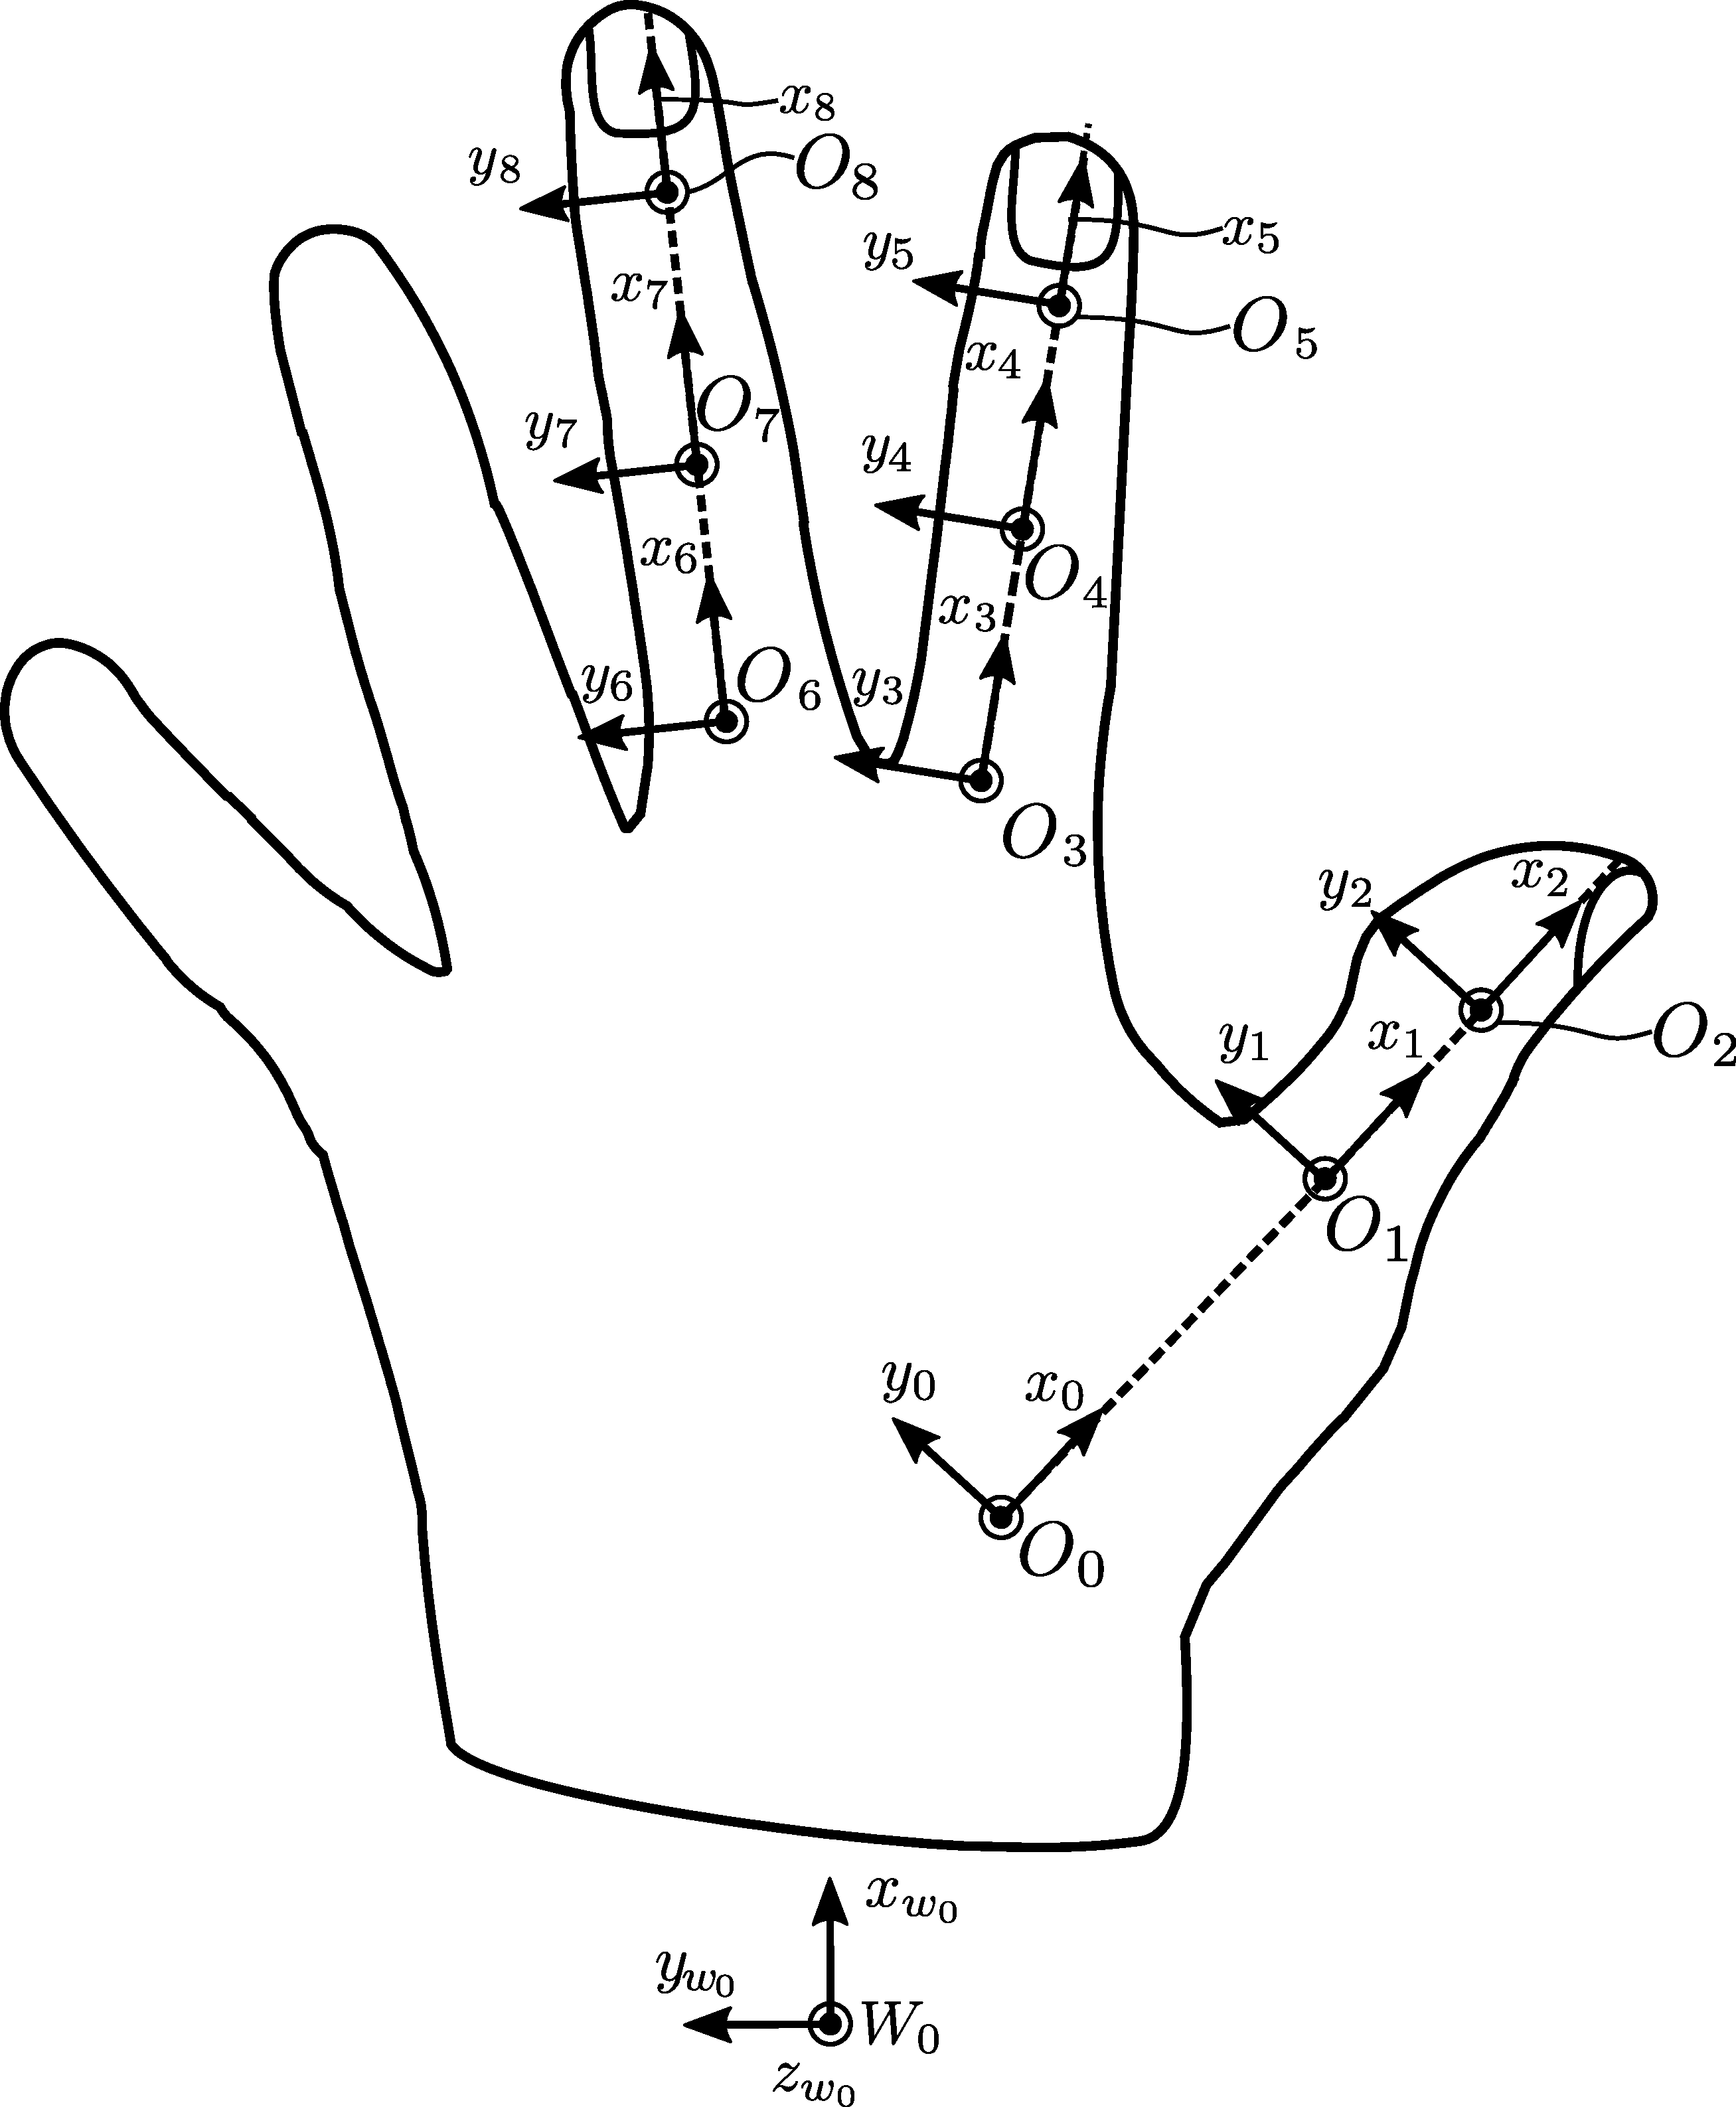
\includegraphics[width=0.45\textwidth]{Figures/kinematic_animation_model.pdf}
        \label{fig:kinematic_animation_model}
    }
    \caption{Orignal kinematic model and animation model.}
    \label{fig:model_comparison_kinematic_animation}
\end{figure}
\subsection{Skeletal Animation}
This application allows the rendering 
of photorealistic deformation of virtual hands, using the
principles of skeletal animation. Using this techique the virtual hand is 
represented in two parts: the mesh which constitutes a realistic 
representation of the geometry and a hierarchical set of interconnected parts
(called bones) that define the motion of the virtual avatar.
Each bone has a three-dimensional transformation from the default bind
pose (which includes its position, scale and orientation), and an optional
parent bone. The bones therefore form a hierarchy. The full transform of a
child node is the product of its parent transform and its own transform.

Each bone in the skeleton is associated with some portion of the character's
visual representation (the mesh) in a process called skinning. In the most
common case of a polygonal mesh character, the bone is associated with a group
of vertices; for example, in a model of a human being, the bone for the
thigh would be associated with the vertices making up the polygons in the
model's thigh. Portions of the character's skin can normally be associated
with multiple bones, each one having a scaling factors called vertex
weights, or blend weights. The movement of skin near the joints of two
bones, can therefore be influenced by both bones. By applying these ideas 
the user can apply direct transformations to the bones of the model and 
produce real-like deformations of the surrounding mesh, see Fig.
\ref{fig:rigged_character}.
\begin{figure}
    \centering
        \subfloat[Surface mesh.]{
        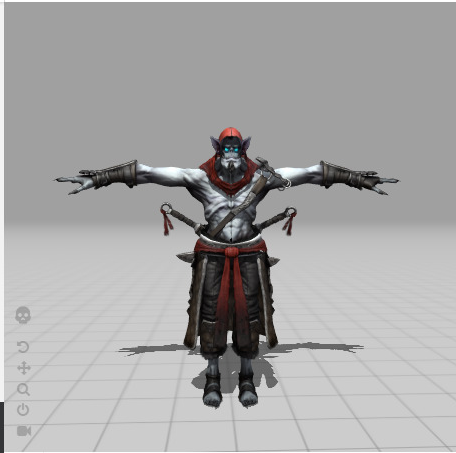
\includegraphics[width=0.45\textwidth]{Figures/character_skin.png}
        \label{fig:character_skin}
    }
    \qquad
    \subfloat[Geometry bones.]{
        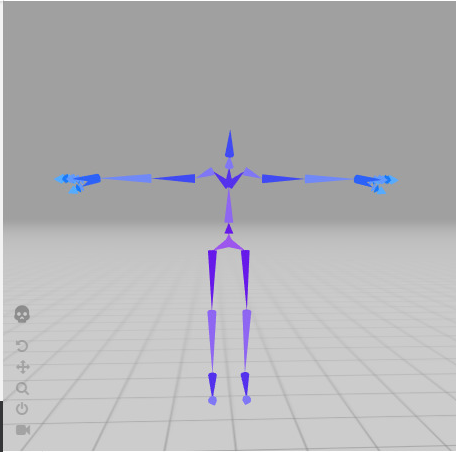
\includegraphics[width=0.45\textwidth]{Figures/character_bones.png}
        \label{fig:character_mesh}
    }
    \qquad
    \subfloat[Rigged character.]{
        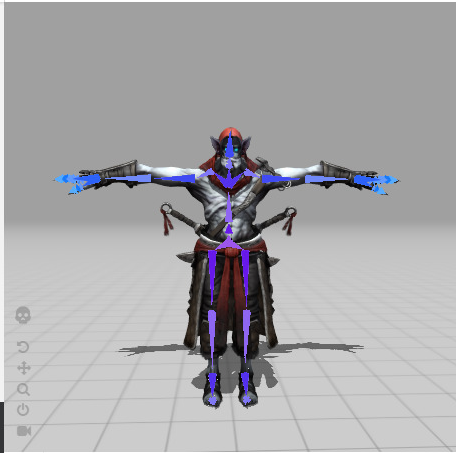
\includegraphics[width=0.45\textwidth]{Figures/character_merged.png}
        \label{fig:character_merged}
    }
    \caption{Steps of skeletal animation.}
    \label{fig:rigged_character}
\end{figure}
In Fig. \ref{fig:hand_bbw} both the internal skeleton and the surrounding 
mesh of the hand is illustrated. Furthermore, the figure presents a color 
map that illustrates the effect of different bones on their surrounding 
mesh vertices. In our application, the weighting and mapping between 
boenes and mesh vertices with the help of the 
bounded biharmonic weight techique. For more information 
on the techique, please see the LibIGL's website and \cite{jacobson_bounded_2011}.
\begin{figure}
    \centering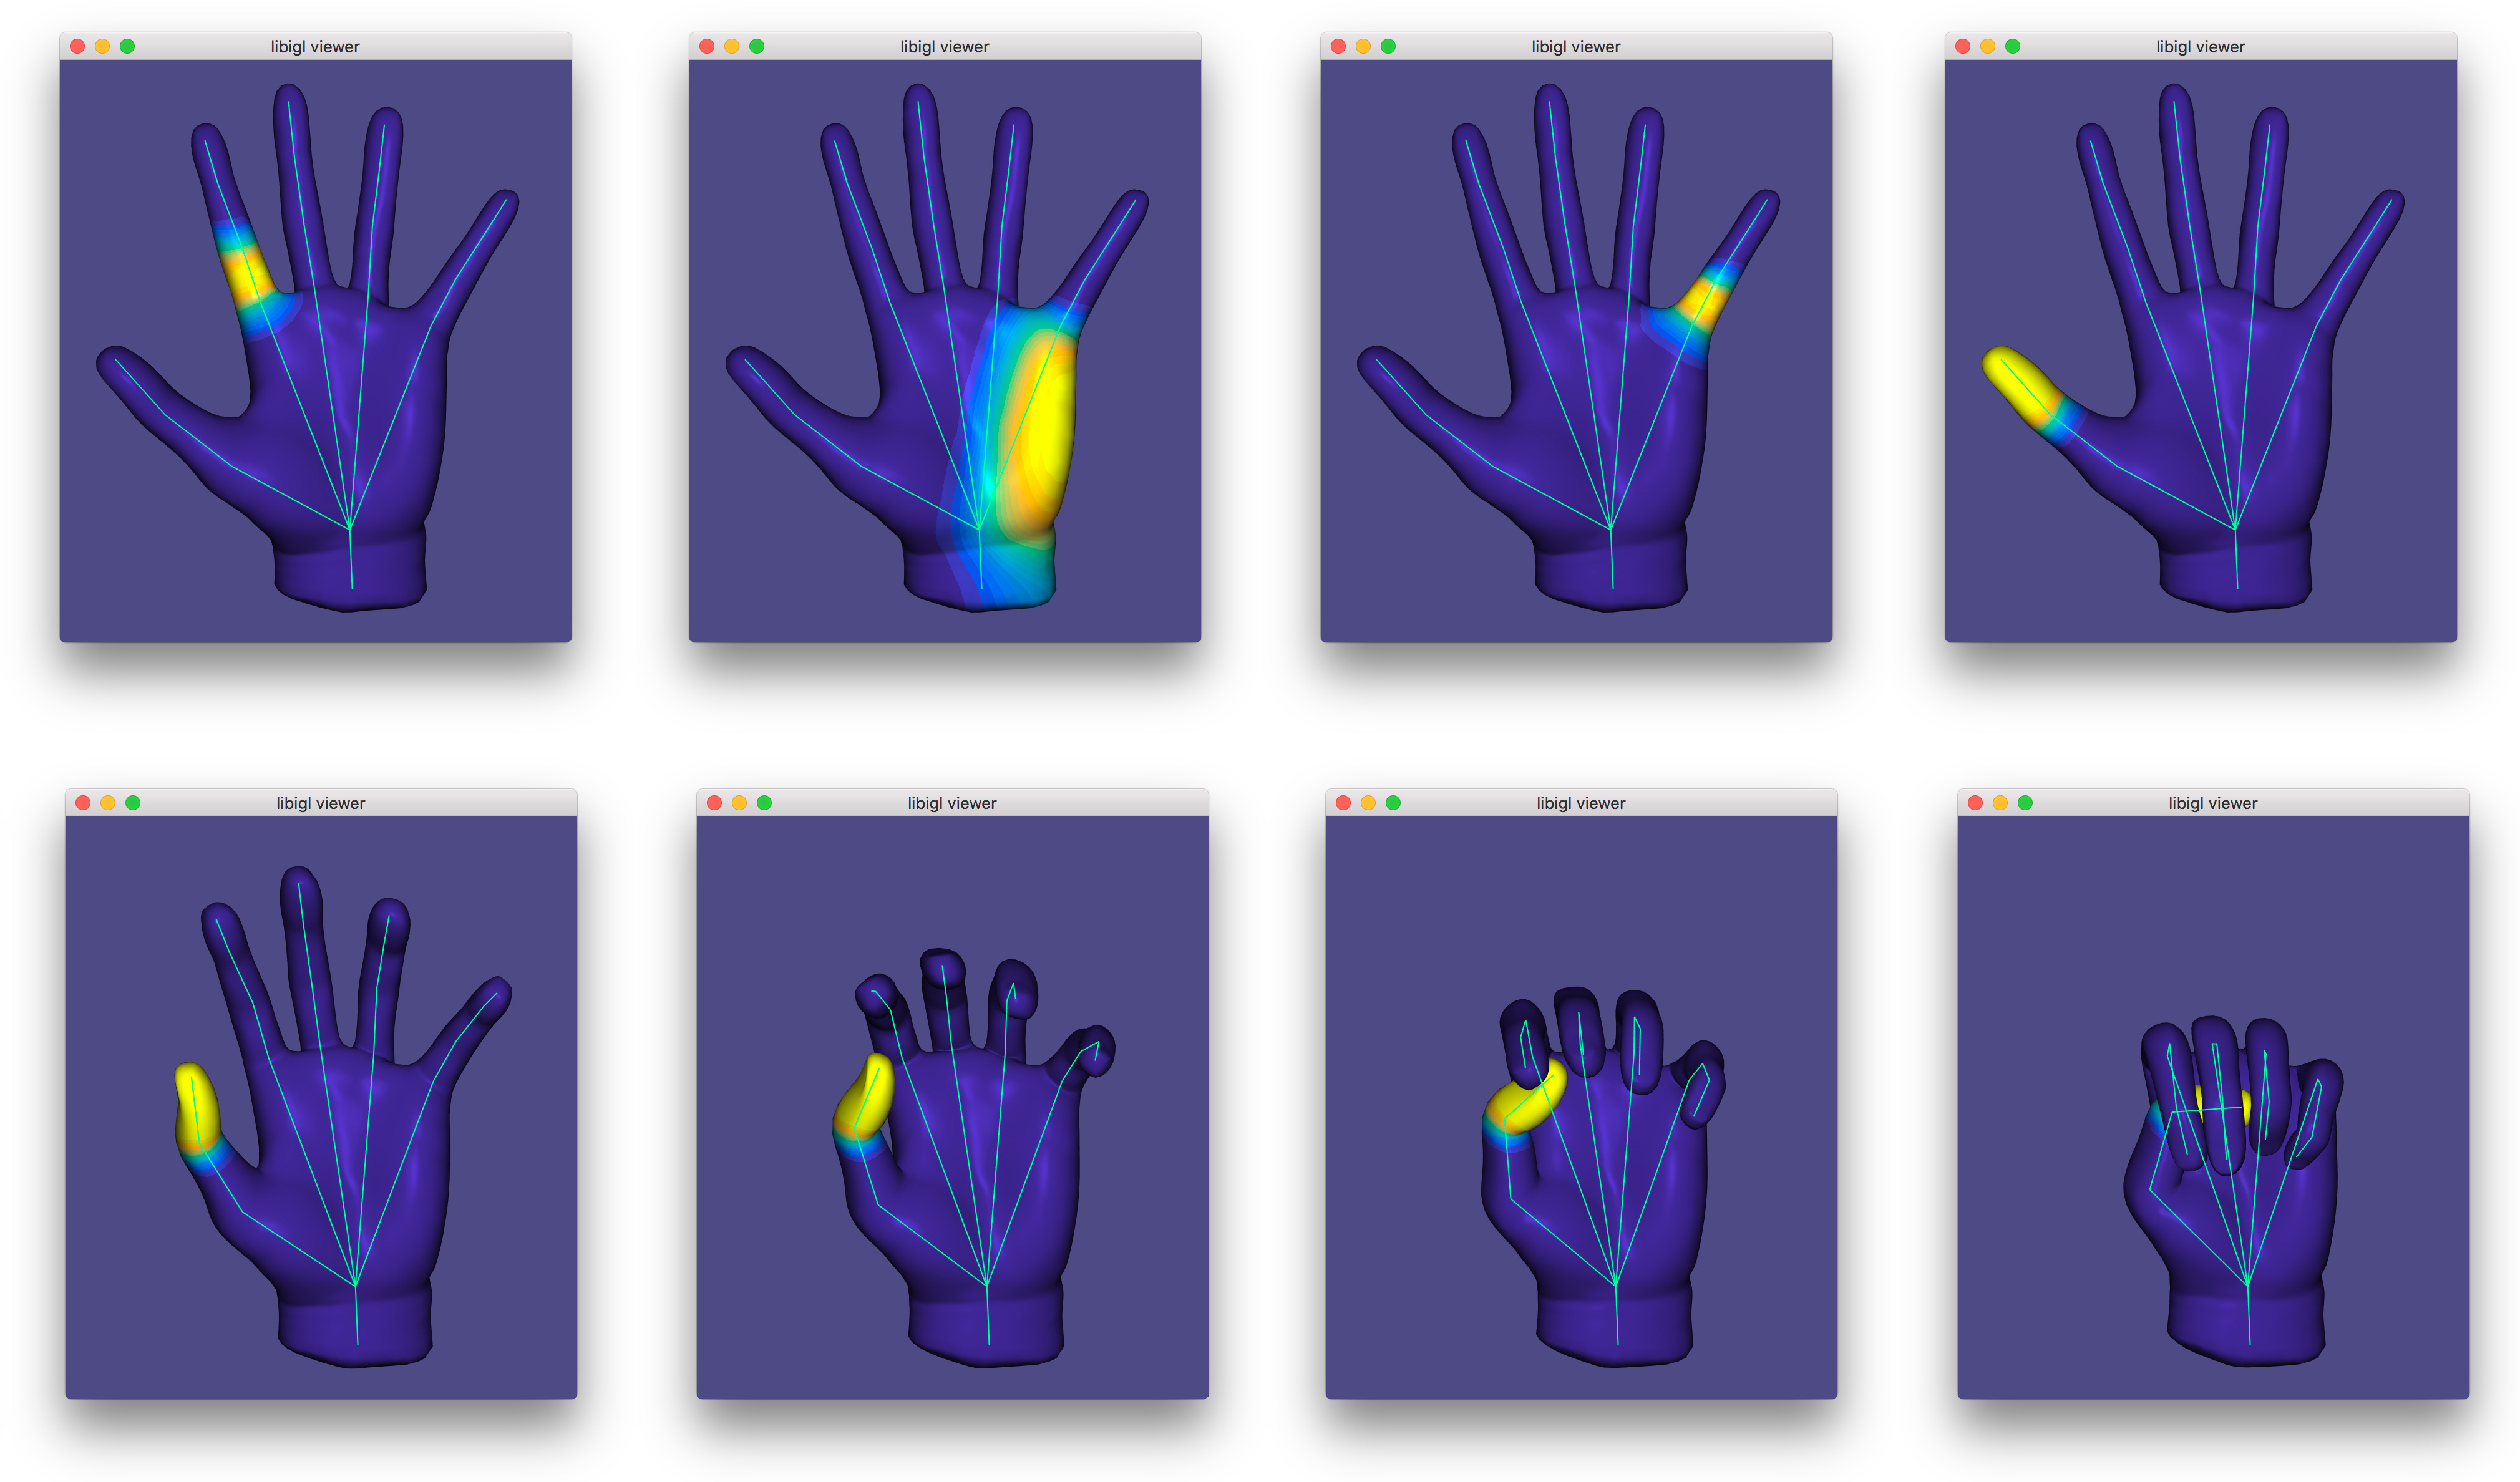
\includegraphics[width=1.0 \linewidth]{Figures/hand_bbw.jpg}
    \caption{Hand rigging and bounded biharmonic weights visualisation.}
    \label{fig:hand_bbw}
\end{figure}
The virtual hand follows the frame convention shown in Fig.
\ref{fig:skeletal_animation_model}.
Again, as shown in Fig \ref{fig:model_comparison_skeletal_animation}
the frames of the skeletal animation differ from the original/basis frame 
convention. However, mapping the configuration of the original kinematic model 
to that of the virtual hand is straightforward. The process is analytically
documented
\texttt{\href{https://amartsop.github.io/SkeletalAnimationMultiThread/classAnimatedHand.html}{here}}.
The source code of the project can be found 
\texttt{\href{https://github.com/amartsop/SkeletalAnimationMultiThread}{here}}
while the full documentation of the application is
\texttt{\href{https://amartsop.github.io/SkeletalAnimationMultiThread/index.html}{here}}.
In Fig. \ref{fig:animation1_capture} we present the rendering result of 
the \texttt{Kinematic Animation Model}.
\begin{figure}[t]
    \centering
        \subfloat[Original kinematic model.]{
        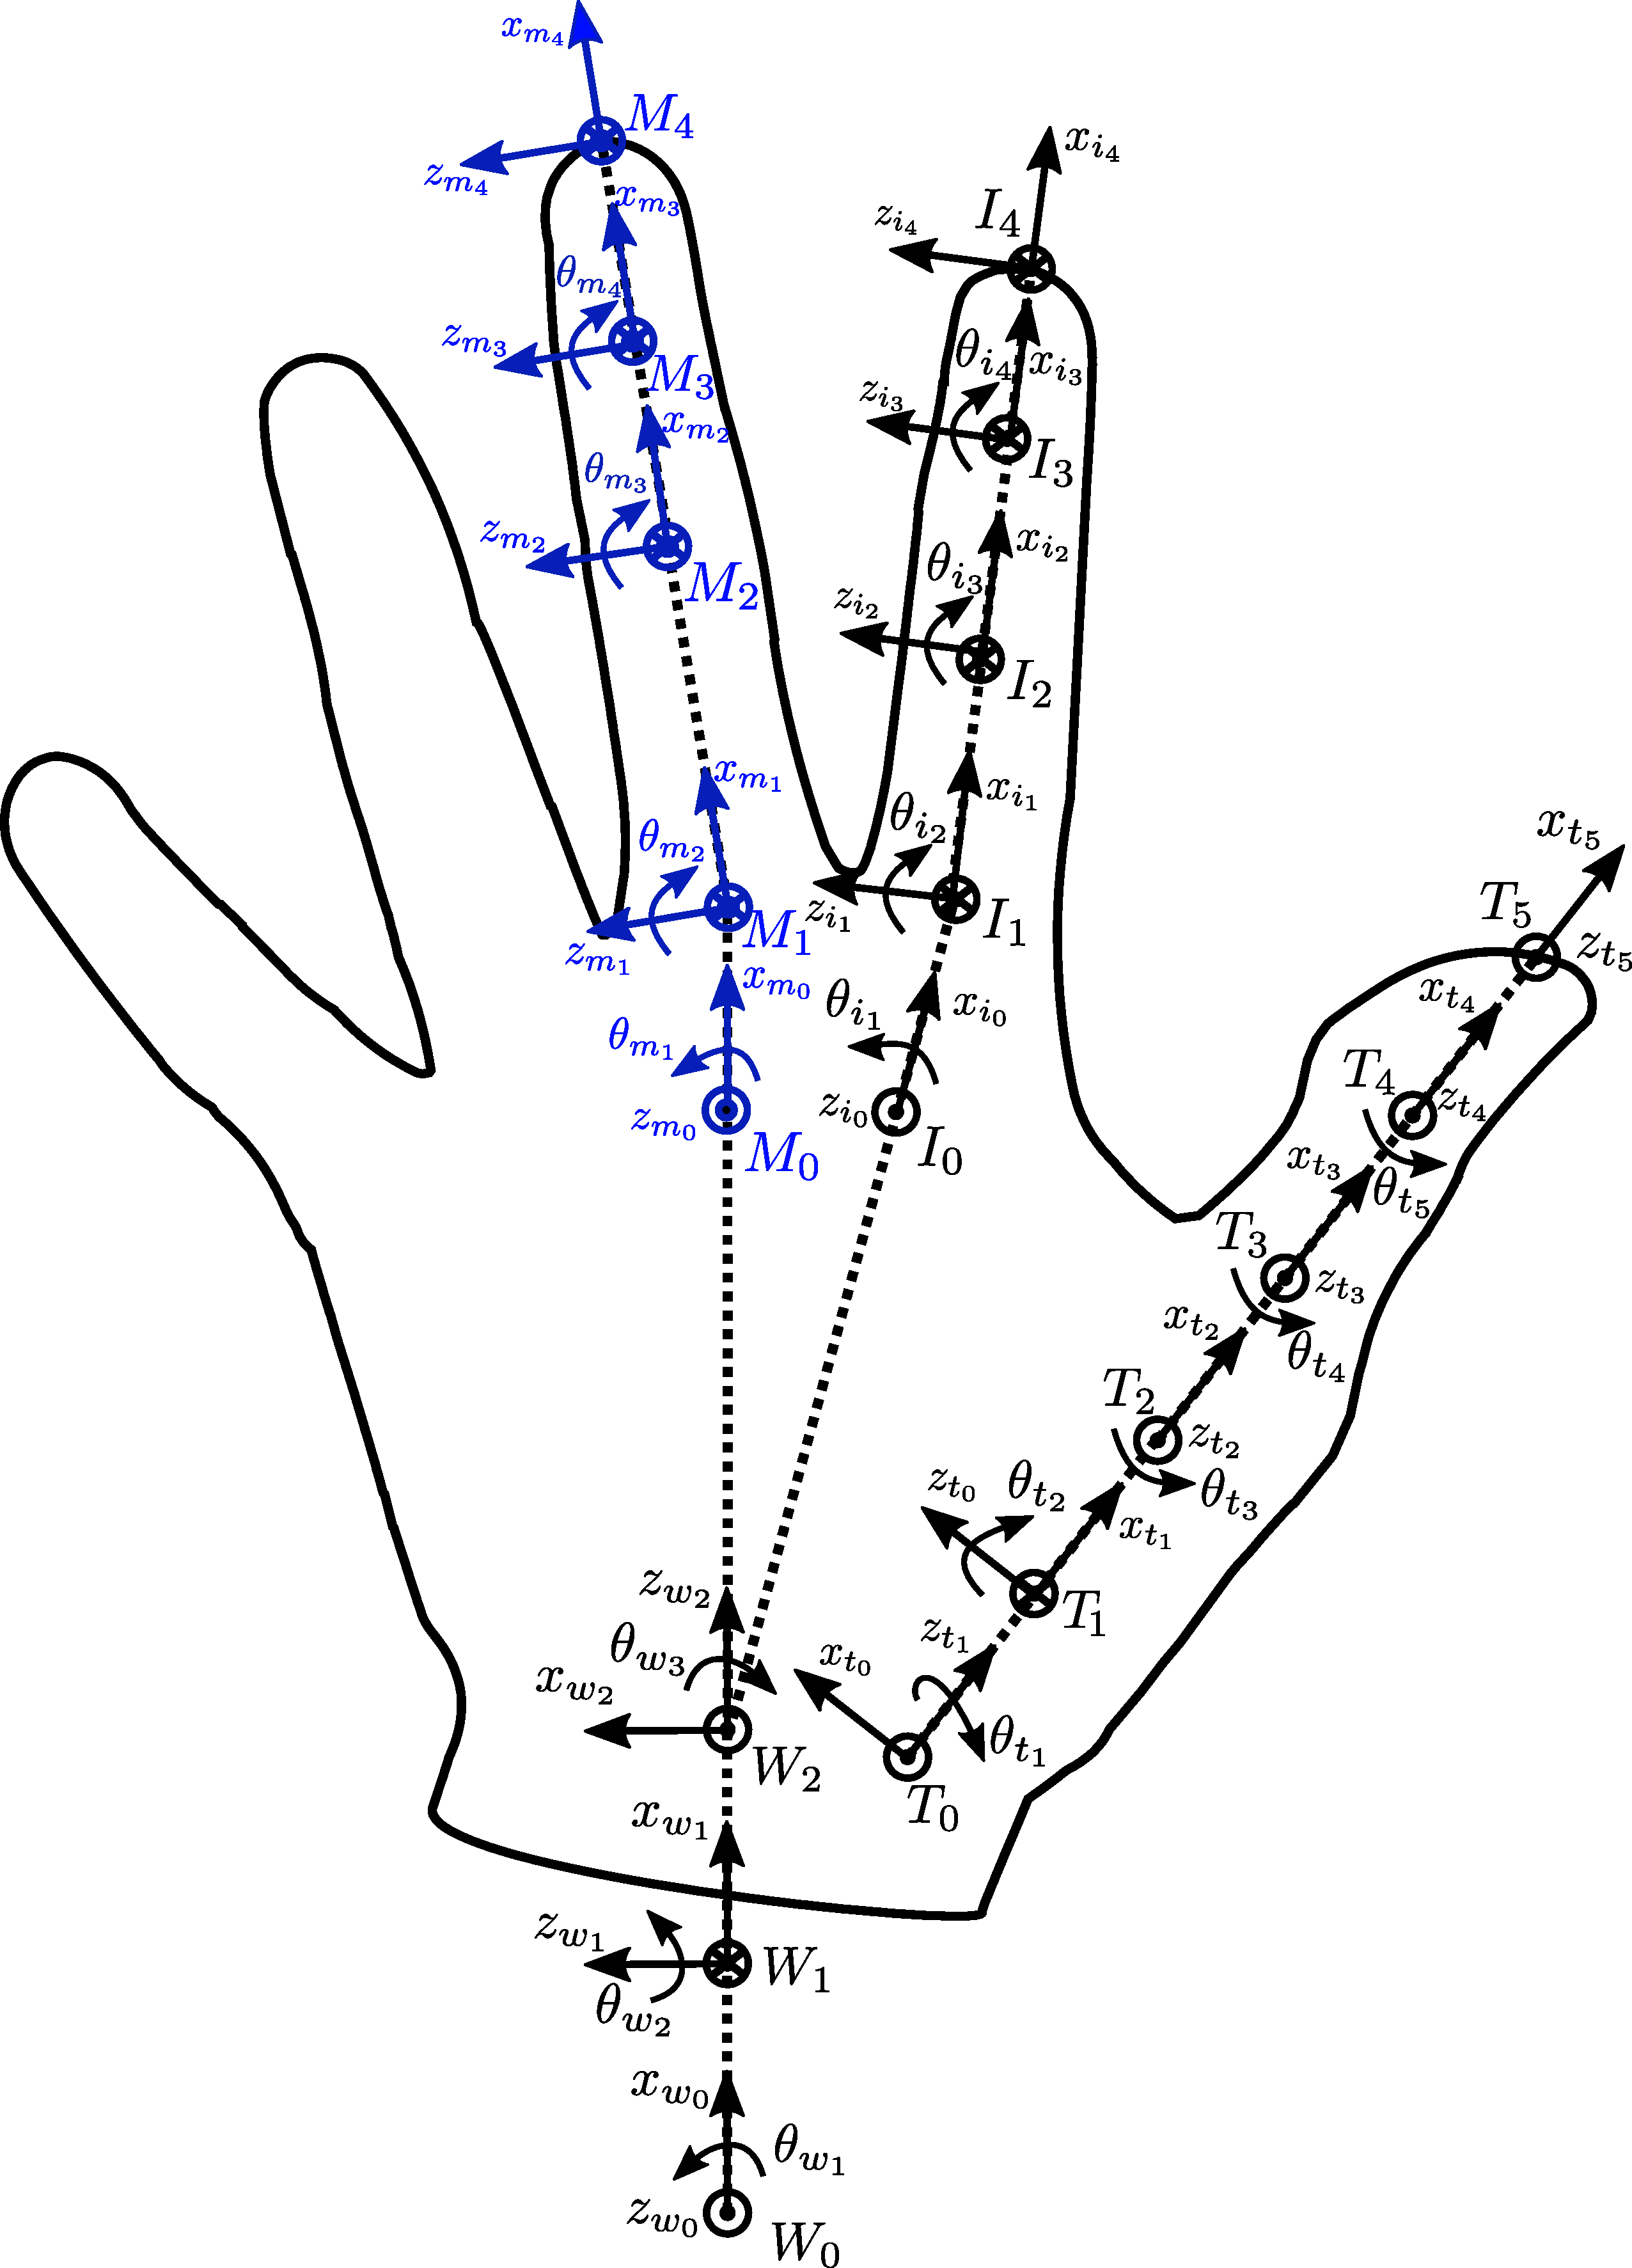
\includegraphics[width=0.45\textwidth]{Figures/kinematic_model.pdf}
        \label{fig:skeletal_model_comparison}
    }
    \qquad
    \subfloat[Skeletal animation model.]{
        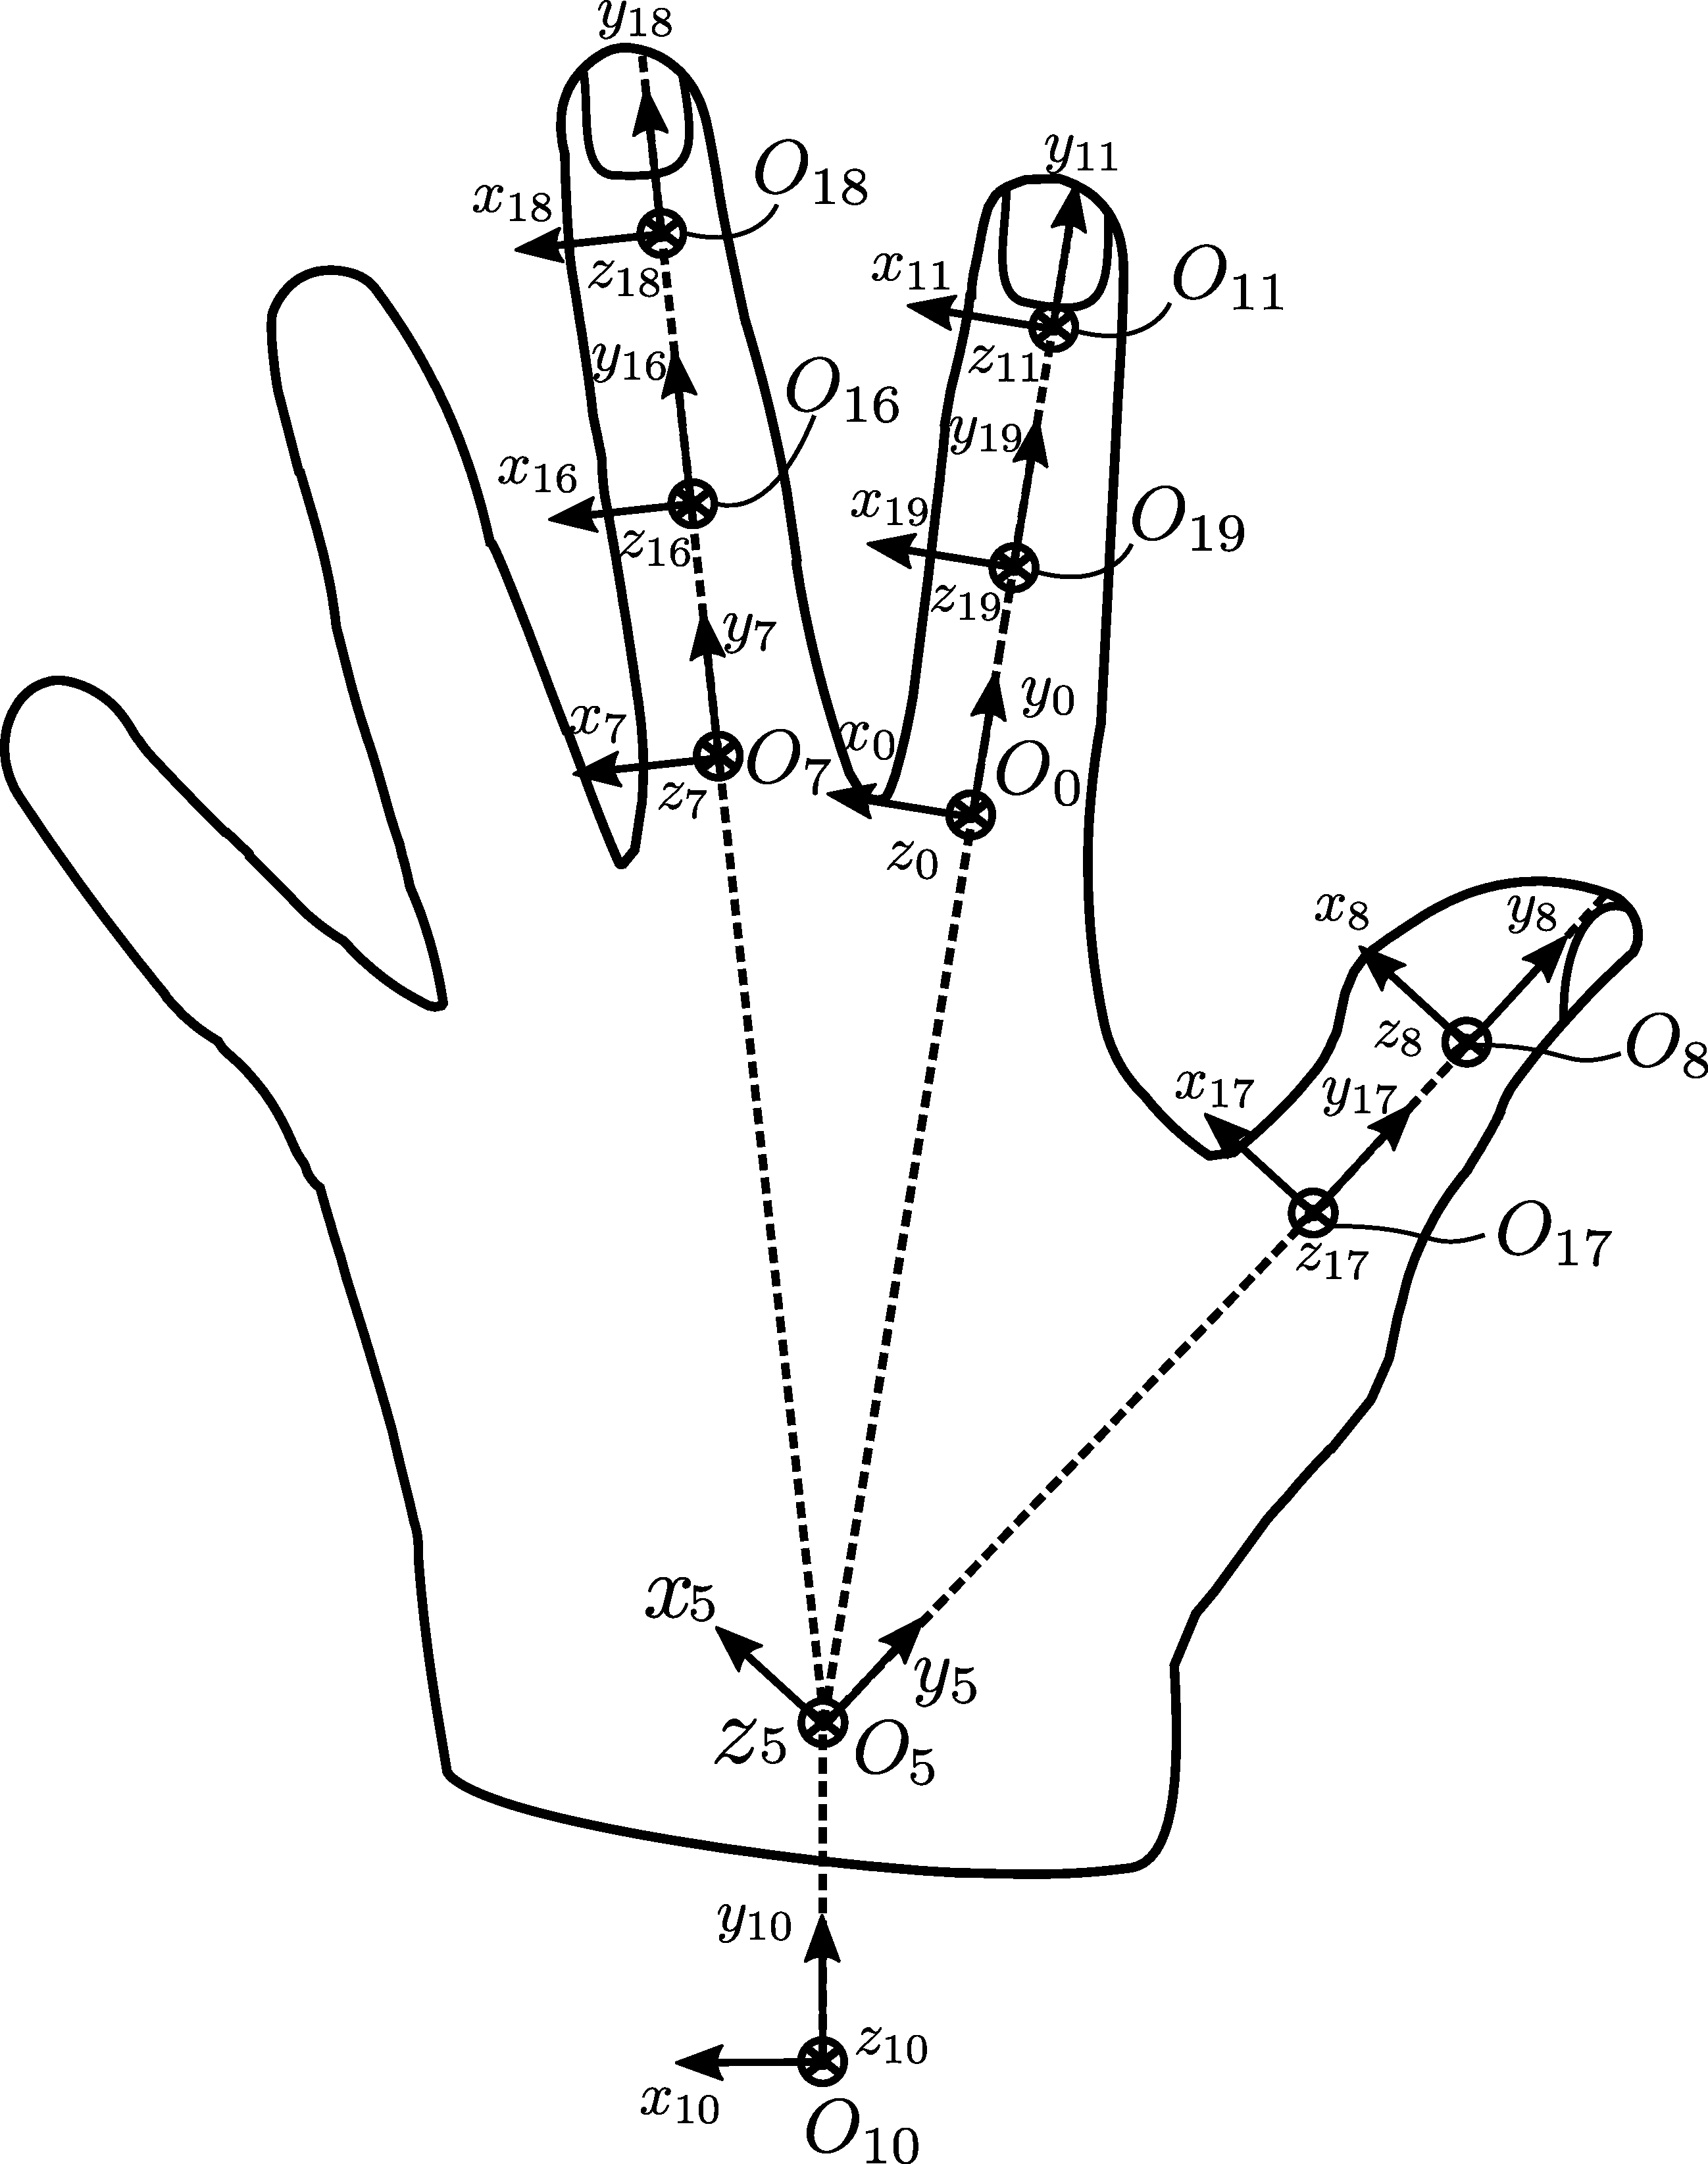
\includegraphics[width=0.45\textwidth]{Figures/skeletal_animation_model.pdf}
        \label{fig:skeletal_animation_model}
    }
    \caption{Orignal kinematic model and skeletal animation model.}
    \label{fig:model_comparison_skeletal_animation}
\end{figure}

\subsection{Face Landmarking}
Our final application is the combination of the Skeletal Animation with 
face landmarking features. As discussed before, for this we have used 
the MediaPipe library, which uses machine learning algorithms for 
identifying 468 unique points that are scattered across the users face.
The points are generated in real-time using a camera stream and they are 
to our rendering application (LibIGL) through means of interprocess
communication. The connectivity relation of the generated vertices is known 
and it is stored as a csv file
\texttt{\href{https://github.com/amartsop/SkeletalAnimationMultiThreadFace/blob/master/share/vertices_connections.csv}{here}}.
The source code of the project can be found 
\texttt{\href{https://github.com/amartsop/SkeletalAnimationMultiThreadFace}{here}}
while the full documentation of the application is
\texttt{\href{https://amartsop.github.io/SkeletalAnimationMultiThreadFace/index.html}{here}}.